% Options for packages loaded elsewhere
\PassOptionsToPackage{unicode}{hyperref}
\PassOptionsToPackage{hyphens}{url}
\PassOptionsToPackage{dvipsnames,svgnames*,x11names*}{xcolor}
%
\documentclass[
]{book}
\usepackage{lmodern}
\usepackage{amssymb,amsmath}
\usepackage{ifxetex,ifluatex}
\ifnum 0\ifxetex 1\fi\ifluatex 1\fi=0 % if pdftex
  \usepackage[T1]{fontenc}
  \usepackage[utf8]{inputenc}
  \usepackage{textcomp} % provide euro and other symbols
\else % if luatex or xetex
  \usepackage{unicode-math}
  \defaultfontfeatures{Scale=MatchLowercase}
  \defaultfontfeatures[\rmfamily]{Ligatures=TeX,Scale=1}
\fi
% Use upquote if available, for straight quotes in verbatim environments
\IfFileExists{upquote.sty}{\usepackage{upquote}}{}
\IfFileExists{microtype.sty}{% use microtype if available
  \usepackage[]{microtype}
  \UseMicrotypeSet[protrusion]{basicmath} % disable protrusion for tt fonts
}{}
\makeatletter
\@ifundefined{KOMAClassName}{% if non-KOMA class
  \IfFileExists{parskip.sty}{%
    \usepackage{parskip}
  }{% else
    \setlength{\parindent}{0pt}
    \setlength{\parskip}{6pt plus 2pt minus 1pt}}
}{% if KOMA class
  \KOMAoptions{parskip=half}}
\makeatother
\usepackage{xcolor}
\IfFileExists{xurl.sty}{\usepackage{xurl}}{} % add URL line breaks if available
\IfFileExists{bookmark.sty}{\usepackage{bookmark}}{\usepackage{hyperref}}
\hypersetup{
  pdftitle={A Collection of Python Examples},
  pdfauthor={Fan Wang},
  colorlinks=true,
  linkcolor=Maroon,
  filecolor=Maroon,
  citecolor=Blue,
  urlcolor=blue,
  pdfcreator={LaTeX via pandoc}}
\urlstyle{same} % disable monospaced font for URLs
\usepackage{color}
\usepackage{fancyvrb}
\newcommand{\VerbBar}{|}
\newcommand{\VERB}{\Verb[commandchars=\\\{\}]}
\DefineVerbatimEnvironment{Highlighting}{Verbatim}{commandchars=\\\{\}}
% Add ',fontsize=\small' for more characters per line
\usepackage{framed}
\definecolor{shadecolor}{RGB}{248,248,248}
\newenvironment{Shaded}{\begin{snugshade}}{\end{snugshade}}
\newcommand{\AlertTok}[1]{\textcolor[rgb]{0.94,0.16,0.16}{#1}}
\newcommand{\AnnotationTok}[1]{\textcolor[rgb]{0.56,0.35,0.01}{\textbf{\textit{#1}}}}
\newcommand{\AttributeTok}[1]{\textcolor[rgb]{0.77,0.63,0.00}{#1}}
\newcommand{\BaseNTok}[1]{\textcolor[rgb]{0.00,0.00,0.81}{#1}}
\newcommand{\BuiltInTok}[1]{#1}
\newcommand{\CharTok}[1]{\textcolor[rgb]{0.31,0.60,0.02}{#1}}
\newcommand{\CommentTok}[1]{\textcolor[rgb]{0.56,0.35,0.01}{\textit{#1}}}
\newcommand{\CommentVarTok}[1]{\textcolor[rgb]{0.56,0.35,0.01}{\textbf{\textit{#1}}}}
\newcommand{\ConstantTok}[1]{\textcolor[rgb]{0.00,0.00,0.00}{#1}}
\newcommand{\ControlFlowTok}[1]{\textcolor[rgb]{0.13,0.29,0.53}{\textbf{#1}}}
\newcommand{\DataTypeTok}[1]{\textcolor[rgb]{0.13,0.29,0.53}{#1}}
\newcommand{\DecValTok}[1]{\textcolor[rgb]{0.00,0.00,0.81}{#1}}
\newcommand{\DocumentationTok}[1]{\textcolor[rgb]{0.56,0.35,0.01}{\textbf{\textit{#1}}}}
\newcommand{\ErrorTok}[1]{\textcolor[rgb]{0.64,0.00,0.00}{\textbf{#1}}}
\newcommand{\ExtensionTok}[1]{#1}
\newcommand{\FloatTok}[1]{\textcolor[rgb]{0.00,0.00,0.81}{#1}}
\newcommand{\FunctionTok}[1]{\textcolor[rgb]{0.00,0.00,0.00}{#1}}
\newcommand{\ImportTok}[1]{#1}
\newcommand{\InformationTok}[1]{\textcolor[rgb]{0.56,0.35,0.01}{\textbf{\textit{#1}}}}
\newcommand{\KeywordTok}[1]{\textcolor[rgb]{0.13,0.29,0.53}{\textbf{#1}}}
\newcommand{\NormalTok}[1]{#1}
\newcommand{\OperatorTok}[1]{\textcolor[rgb]{0.81,0.36,0.00}{\textbf{#1}}}
\newcommand{\OtherTok}[1]{\textcolor[rgb]{0.56,0.35,0.01}{#1}}
\newcommand{\PreprocessorTok}[1]{\textcolor[rgb]{0.56,0.35,0.01}{\textit{#1}}}
\newcommand{\RegionMarkerTok}[1]{#1}
\newcommand{\SpecialCharTok}[1]{\textcolor[rgb]{0.00,0.00,0.00}{#1}}
\newcommand{\SpecialStringTok}[1]{\textcolor[rgb]{0.31,0.60,0.02}{#1}}
\newcommand{\StringTok}[1]{\textcolor[rgb]{0.31,0.60,0.02}{#1}}
\newcommand{\VariableTok}[1]{\textcolor[rgb]{0.00,0.00,0.00}{#1}}
\newcommand{\VerbatimStringTok}[1]{\textcolor[rgb]{0.31,0.60,0.02}{#1}}
\newcommand{\WarningTok}[1]{\textcolor[rgb]{0.56,0.35,0.01}{\textbf{\textit{#1}}}}
\usepackage{longtable,booktabs}
% Correct order of tables after \paragraph or \subparagraph
\usepackage{etoolbox}
\makeatletter
\patchcmd\longtable{\par}{\if@noskipsec\mbox{}\fi\par}{}{}
\makeatother
% Allow footnotes in longtable head/foot
\IfFileExists{footnotehyper.sty}{\usepackage{footnotehyper}}{\usepackage{footnote}}
\makesavenoteenv{longtable}
\usepackage{graphicx,grffile}
\makeatletter
\def\maxwidth{\ifdim\Gin@nat@width>\linewidth\linewidth\else\Gin@nat@width\fi}
\def\maxheight{\ifdim\Gin@nat@height>\textheight\textheight\else\Gin@nat@height\fi}
\makeatother
% Scale images if necessary, so that they will not overflow the page
% margins by default, and it is still possible to overwrite the defaults
% using explicit options in \includegraphics[width, height, ...]{}
\setkeys{Gin}{width=\maxwidth,height=\maxheight,keepaspectratio}
% Set default figure placement to htbp
\makeatletter
\def\fps@figure{htbp}
\makeatother
\setlength{\emergencystretch}{3em} % prevent overfull lines
\providecommand{\tightlist}{%
  \setlength{\itemsep}{0pt}\setlength{\parskip}{0pt}}
\setcounter{secnumdepth}{5}
\usepackage{bbm}
\usepackage{booktabs}
\usepackage{longtable}
\usepackage{array}
\usepackage{multirow}
\usepackage{wrapfig}
\usepackage{float}
% \floatplacement{figure}{H}
\usepackage[labelformat = empty]{caption}
\usepackage{colortbl}
\usepackage{pdflscape}
\usepackage{tabu}
\usepackage{threeparttable}
\usepackage{threeparttablex}
\usepackage[normalem]{ulem}
\usepackage{makecell}
\usepackage{xcolor}
\usepackage{geometry}
\geometry{
	a4paper,
	left=1.0in,
	right=1.0in,
	top=1.0in,
	bottom=1.0in,
}
\setcounter{secnumdepth}{5}
\setcounter{tocdepth}{5}
\usepackage[]{natbib}
\bibliographystyle{apalike}

\title{A Collection of Python Examples}
\author{Fan Wang}
\date{2020-06-23}

\begin{document}
\maketitle

{
\hypersetup{linkcolor=}
\setcounter{tocdepth}{2}
\tableofcontents
}
\hypertarget{preface}{%
\chapter*{Preface}\label{preface}}
\addcontentsline{toc}{chapter}{Preface}

The work-in-progress \href{https://github.com/FanWangEcon/pyfan}{pyfan} repository contains:

\begin{enumerate}
\def\labelenumi{\arabic{enumi}.}
\tightlist
\item
  Tutorials and examples for various research tasks: \href{https://fanwangecon.github.io/pyfan/bookdown}{\textbf{bookdown site}} and \href{https://fanwangecon.github.io/pyfan/bookdown/A-Collection-of-Python-Examples.pdf}{\textbf{bookdown pdf}}.
\item
  A package for basic data, graph and research tasks: \href{https://pyfan.readthedocs.io/en/latest/}{\textbf{readthedocs}} and \href{https://pypi.org/project/pyfan/}{\textbf{pypi}}.
\end{enumerate}

Materials are gathered from various \href{https://fanwangecon.github.io/research}{projects} in which python code is used for research and paper-administrative tasks. Files are from \href{https://fanwangecon.github.io/}{\textbf{Fan}}'s \href{https://github.com/FanWangEcon/pyfan}{pyfan} repository which has an associated \href{https://pypi.org/project/pyfan/}{package}. The package functionalize various tasks tested out in the Rmd files. In addition, the \href{https://github.com/FanWangEcon/pyecon}{pyecon} repository and the associated \href{https://pypi.org/project/pyecon/}{package} (\href{https://pyfan.readthedocs.io/en/latest/autoapi/pyfan/index.html\#module-pyfan}{readthedocs}) contain functions and rmd files related explicitly to solving economic models.

From \href{https://fanwangecon.github.io/}{Fan}'s other repositories: For dynamic borrowing and savings problems, see \href{https://fanwangecon.github.io/CodeDynaAsset/}{Dynamic Asset Repository (Matlab)}; For code examples, see also \href{https://fanwangecon.github.io/M4Econ/}{Matlab Example Code}, \href{https://fanwangecon.github.io/R4Econ/}{R Example Code}, and \href{https://fanwangecon.github.io/Stata4Econ/}{Stata Example Code}; For intro econ with Matlab, see \href{https://fanwangecon.github.io/Math4Econ/}{Intro Mathematics for Economists}, and for intro stat with R, see \href{https://fanwangecon.github.io/Stat4Econ/}{Intro Statistics for Undergraduates}. See \href{https://github.com/FanWangEcon}{here} for all of \href{https://fanwangecon.github.io/}{Fan}'s public repositories.

The site is built using \href{https://bookdown.org/}{Bookdown} \citep{R-bookdown}.

Please contact \href{https://fanwangecon.github.io/}{FanWangEcon} for issues or problems.

\hypertarget{array-matrix-dataframe}{%
\chapter{Array, Matrix, Dataframe}\label{array-matrix-dataframe}}

\hypertarget{array}{%
\section{Array}\label{array}}

\hypertarget{strings}{%
\subsection{Strings}\label{strings}}

\begin{quote}
Go back to \href{http://fanwangecon.github.io/}{fan}'s \href{https://fanwangecon.github.io/pyfan/}{Python Code Examples} Repository (\href{https://fanwangecon.github.io/pyfan/bookdown}{bookdown site}).
\end{quote}

\hypertarget{search-if-names-include-strings}{%
\subsubsection{Search if Names Include Strings}\label{search-if-names-include-strings}}

Given a list of strings, loop but skip if string contains elements string list.

\begin{Shaded}
\begin{Highlighting}[]
\CommentTok{# define string}
\NormalTok{ls_st_ignore }\OperatorTok{=}\NormalTok{ [}\StringTok{'abc'}\NormalTok{, }\StringTok{'efg'}\NormalTok{, }\StringTok{'xyz'}\NormalTok{]}
\NormalTok{ls_st_loop }\OperatorTok{=}\NormalTok{ [}\StringTok{'ab cefg sdf'}\NormalTok{, }\StringTok{'12345'}\NormalTok{, }\StringTok{'xyz'}\NormalTok{, }\StringTok{'abc xyz'}\NormalTok{, }\StringTok{'good morning'}\NormalTok{]}

\CommentTok{# zip and loop and replace}
\ControlFlowTok{for}\NormalTok{ st_loop }\KeywordTok{in}\NormalTok{ ls_st_loop:}
  \ControlFlowTok{if} \BuiltInTok{sum}\NormalTok{([st_ignore }\KeywordTok{in}\NormalTok{ st_loop }\ControlFlowTok{for}\NormalTok{ st_ignore }\KeywordTok{in}\NormalTok{ ls_st_ignore]):}
    \BuiltInTok{print}\NormalTok{(}\StringTok{'skip:'}\NormalTok{, st_loop)}
  \ControlFlowTok{else}\NormalTok{:}
    \BuiltInTok{print}\NormalTok{(}\StringTok{'not skip:'}\NormalTok{, st_loop)}
\end{Highlighting}
\end{Shaded}

\begin{verbatim}
## skip: ab cefg sdf
## not skip: 12345
## skip: xyz
## skip: abc xyz
## not skip: good morning
\end{verbatim}

\hypertarget{replace-a-set-of-strings-in-string}{%
\subsubsection{Replace a Set of Strings in String}\label{replace-a-set-of-strings-in-string}}

Replace terms in string

\begin{Shaded}
\begin{Highlighting}[]
\CommentTok{# define string}
\NormalTok{st_full }\OperatorTok{=} \StringTok{"""}
\StringTok{abc is a great efg, probably xyz. Yes, xyz is great, like efg. }
\StringTok{eft good, EFG capitalized, efg good again. }
\StringTok{A B C or abc or ABC. Interesting xyz. }
\StringTok{"""}

\CommentTok{# define new and old}
\NormalTok{ls_st_old }\OperatorTok{=}\NormalTok{ [}\StringTok{'abc'}\NormalTok{, }\StringTok{'efg'}\NormalTok{, }\StringTok{'xyz'}\NormalTok{]}
\NormalTok{ls_st_new }\OperatorTok{=}\NormalTok{ [}\StringTok{'123'}\NormalTok{, }\StringTok{'456'}\NormalTok{, }\StringTok{'789'}\NormalTok{]}

\CommentTok{# zip and loop and replace}
\ControlFlowTok{for}\NormalTok{ old, new }\KeywordTok{in} \BuiltInTok{zip}\NormalTok{(ls_st_old, ls_st_new):}
\NormalTok{  st_full }\OperatorTok{=}\NormalTok{ st_full.replace(old, new)}

\CommentTok{# print}
\BuiltInTok{print}\NormalTok{(st_full)}
\end{Highlighting}
\end{Shaded}

\begin{verbatim}
## 
## 123 is a great 456, probably 789. Yes, 789 is great, like 456. 
## eft good, EFG capitalized, 456 good again. 
## A B C or 123 or ABC. Interesting 789.
\end{verbatim}

\hypertarget{wrap-string-with-fixed-width}{%
\subsubsection{Wrap String with Fixed Width}\label{wrap-string-with-fixed-width}}

Given a long string, wrap it into multiple lines with fixed width.

\begin{Shaded}
\begin{Highlighting}[]
\ImportTok{import}\NormalTok{ textwrap}

\CommentTok{# A long Path}
\NormalTok{st_path }\OperatorTok{=} \StringTok{"""}
\StringTok{C:/Users/fan/Documents/Dropbox (UH-ECON)/Project Emily Minority Survey/EthLang/reg_lang_abi_cls_mino/tab3_fm/attain_m_vs_f/tab3_mand_talk_m2c_hfracle02.tex}
\StringTok{"""}

\CommentTok{# Wrap text with tight width}
\NormalTok{st_wrapped }\OperatorTok{=}\NormalTok{ textwrap.fill(st_path, width }\OperatorTok{=} \DecValTok{20}\NormalTok{)}
\BuiltInTok{print}\NormalTok{(st_wrapped)}
\end{Highlighting}
\end{Shaded}

\begin{verbatim}
##  C:/Users/fan/Docume
## nts/Dropbox (UH-
## ECON)/Project Emily
## Minority Survey/EthL
## ang/reg_lang_abi_cls
## _mino/tab3_fm/attain
## _m_vs_f/tab3_mand_ta
## lk_m2c_hfracle02.tex
\end{verbatim}

Combine Strings that are wrapped and not Wrapped

\begin{Shaded}
\begin{Highlighting}[]

\CommentTok{# Paths}
\NormalTok{st_path_a }\OperatorTok{=} \StringTok{"C:/Users/fan/Documents/Dropbox (UH-ECON)/Project Emily Minority Survey/EthLang/reg_lang_abi_cls_mino/tab3_fm/attain_m_vs_f/tab3_mand_talk_m2c_hfracle02.tex"}
\NormalTok{st_path_b }\OperatorTok{=} \StringTok{'C:/Users/fan/R4Econ/support/development/fs_packaging.html'}

\CommentTok{# Combine Strings and Wrap}
\NormalTok{str_dc_records }\OperatorTok{=} \StringTok{'First Path:'}\NormalTok{.upper() }\OperatorTok{+} \StringTok{'}\CharTok{\textbackslash{}n}\StringTok{'} \OperatorTok{+} \OperatorTok{\textbackslash{}}
\NormalTok{                 textwrap.fill(st_path_a, width}\OperatorTok{=}\DecValTok{25}\NormalTok{) }\OperatorTok{+} \StringTok{'}\CharTok{\textbackslash{}n\textbackslash{}n}\StringTok{'} \OperatorTok{+} \OperatorTok{\textbackslash{}}
                 \CommentTok{'Second Path:'}\NormalTok{.upper() }\OperatorTok{+} \StringTok{'}\CharTok{\textbackslash{}n}\StringTok{'} \OperatorTok{+} \OperatorTok{\textbackslash{}}
\NormalTok{                 textwrap.fill(st_path_b, width}\OperatorTok{=}\DecValTok{25}\NormalTok{)}
              
\CommentTok{# Print}
\BuiltInTok{print}\NormalTok{(str_dc_records)                 }
\end{Highlighting}
\end{Shaded}

\begin{verbatim}
## FIRST PATH:
## C:/Users/fan/Documents/Dr
## opbox (UH-ECON)/Project
## Emily Minority Survey/Eth
## Lang/reg_lang_abi_cls_min
## o/tab3_fm/attain_m_vs_f/t
## ab3_mand_talk_m2c_hfracle
## 02.tex
## 
## SECOND PATH:
## C:/Users/fan/R4Econ/suppo
## rt/development/fs_packagi
## ng.html
\end{verbatim}

\hypertarget{dictionary}{%
\section{Dictionary}\label{dictionary}}

\hypertarget{dictionary-1}{%
\subsection{Dictionary}\label{dictionary-1}}

\begin{quote}
Go back to \href{http://fanwangecon.github.io/}{fan}'s \href{https://fanwangecon.github.io/pyfan/}{Python Code Examples} Repository (\href{https://fanwangecon.github.io/pyfan/bookdown}{bookdown site}).
\end{quote}

\hypertarget{create-a-list-of-dictionaries}{%
\subsubsection{Create a List of Dictionaries}\label{create-a-list-of-dictionaries}}

\begin{Shaded}
\begin{Highlighting}[]
\ImportTok{import}\NormalTok{ datetime}
\ImportTok{import}\NormalTok{ pprint}
\NormalTok{ls_dc_exa }\OperatorTok{=}\NormalTok{  [}
\NormalTok{    \{}\StringTok{"file"}\NormalTok{: }\StringTok{"mat_matlab"}\NormalTok{,}
     \StringTok{"title"}\NormalTok{: }\StringTok{"One Variable Graphs and Tables"}\NormalTok{,}
     \StringTok{"description"}\NormalTok{: }\StringTok{"Frequency table, bar chart and histogram"}\NormalTok{,}
     \StringTok{"val"}\NormalTok{: }\DecValTok{1}\NormalTok{,}
     \StringTok{"date"}\NormalTok{: datetime.date(}\DecValTok{2020}\NormalTok{, }\DecValTok{5}\NormalTok{, }\DecValTok{2}\NormalTok{)\},}
\NormalTok{    \{}\StringTok{"file"}\NormalTok{: }\StringTok{"mat_two"}\NormalTok{,}
     \StringTok{"title"}\NormalTok{: }\StringTok{"Second file"}\NormalTok{,}
     \StringTok{"description"}\NormalTok{: }\StringTok{"Second file."}\NormalTok{,}
     \StringTok{"val"}\NormalTok{: [}\DecValTok{1}\NormalTok{, }\DecValTok{2}\NormalTok{, }\DecValTok{3}\NormalTok{],}
     \StringTok{"date"}\NormalTok{: datetime.date(}\DecValTok{2020}\NormalTok{, }\DecValTok{5}\NormalTok{, }\DecValTok{2}\NormalTok{)\},}
\NormalTok{    \{}\StringTok{"file"}\NormalTok{: }\StringTok{"mat_algebra_rules"}\NormalTok{,}
     \StringTok{"title"}\NormalTok{: }\StringTok{"Opening a Dataset"}\NormalTok{,}
     \StringTok{"description"}\NormalTok{: }\StringTok{"Opening a Dataset."}\NormalTok{,}
     \StringTok{"val"}\NormalTok{: }\FloatTok{1.1}\NormalTok{,}
     \StringTok{"date"}\NormalTok{: datetime.date(}\DecValTok{2018}\NormalTok{, }\DecValTok{12}\NormalTok{, }\DecValTok{1}\NormalTok{)\}}
\NormalTok{]}
\NormalTok{pprint.pprint(ls_dc_exa, width}\OperatorTok{=}\DecValTok{1}\NormalTok{)}
\end{Highlighting}
\end{Shaded}

\begin{verbatim}
## [{'date': datetime.date(2020, 5, 2),
##   'description': 'Frequency '
##                  'table, '
##                  'bar '
##                  'chart '
##                  'and '
##                  'histogram',
##   'file': 'mat_matlab',
##   'title': 'One '
##            'Variable '
##            'Graphs '
##            'and '
##            'Tables',
##   'val': 1},
##  {'date': datetime.date(2020, 5, 2),
##   'description': 'Second '
##                  'file.',
##   'file': 'mat_two',
##   'title': 'Second '
##            'file',
##   'val': [1,
##           2,
##           3]},
##  {'date': datetime.date(2018, 12, 1),
##   'description': 'Opening '
##                  'a '
##                  'Dataset.',
##   'file': 'mat_algebra_rules',
##   'title': 'Opening '
##            'a '
##            'Dataset',
##   'val': 1.1}]
\end{verbatim}

\hypertarget{iteratively-add-to-a-dictionary}{%
\subsubsection{Iteratively Add to A Dictionary}\label{iteratively-add-to-a-dictionary}}

Iteratively add additional Key and Value pairs to a dictionary.

\begin{Shaded}
\begin{Highlighting}[]

\NormalTok{ls_snm_tex }\OperatorTok{=}\NormalTok{ [}\StringTok{"file1.tex"}\NormalTok{, }\StringTok{"file2.tex"}\NormalTok{, }\StringTok{"file3.tex"}\NormalTok{]}
\NormalTok{ls_snm_pdf }\OperatorTok{=}\NormalTok{ [}\StringTok{"file1.pdf"}\NormalTok{, }\StringTok{"file2.pdf"}\NormalTok{, }\StringTok{"file3.pdf"}\NormalTok{]}

\NormalTok{dc_tex_pdf }\OperatorTok{=}\NormalTok{ \{\}}
\ControlFlowTok{for}\NormalTok{ tex, pdf }\KeywordTok{in} \BuiltInTok{zip}\NormalTok{(ls_snm_tex, ls_snm_pdf):}
\NormalTok{  dc_tex_pdf[tex] }\OperatorTok{=}\NormalTok{ pdf}

\NormalTok{pprint.pprint(dc_tex_pdf, width}\OperatorTok{=}\DecValTok{1}\NormalTok{)}
\end{Highlighting}
\end{Shaded}

\begin{verbatim}
## {'file1.tex': 'file1.pdf',
##  'file2.tex': 'file2.pdf',
##  'file3.tex': 'file3.pdf'}
\end{verbatim}

\hypertarget{select-by-keys-in-dictionary}{%
\subsubsection{Select by Keys in Dictionary}\label{select-by-keys-in-dictionary}}

Given a list of dictionary, search if key name is in list:

\begin{Shaded}
\begin{Highlighting}[]
\CommentTok{# string to search through}
\NormalTok{ls_str_file_ids }\OperatorTok{=}\NormalTok{ [}\StringTok{'mat_matlab'}\NormalTok{, }\StringTok{'mat_algebra_rules'}\NormalTok{]}
\CommentTok{# select subset}
\NormalTok{ls_dc_selected }\OperatorTok{=}\NormalTok{ [dc_exa}
                  \ControlFlowTok{for}\NormalTok{ dc_exa }\KeywordTok{in}\NormalTok{ ls_dc_exa}
                  \ControlFlowTok{if}\NormalTok{ dc_exa[}\StringTok{'file'}\NormalTok{] }\KeywordTok{in}\NormalTok{ ls_str_file_ids]}
\CommentTok{# print}
\NormalTok{pprint.pprint(ls_dc_selected, width}\OperatorTok{=}\DecValTok{1}\NormalTok{)}
\end{Highlighting}
\end{Shaded}

\begin{verbatim}
## [{'date': datetime.date(2020, 5, 2),
##   'description': 'Frequency '
##                  'table, '
##                  'bar '
##                  'chart '
##                  'and '
##                  'histogram',
##   'file': 'mat_matlab',
##   'title': 'One '
##            'Variable '
##            'Graphs '
##            'and '
##            'Tables',
##   'val': 1},
##  {'date': datetime.date(2018, 12, 1),
##   'description': 'Opening '
##                  'a '
##                  'Dataset.',
##   'file': 'mat_algebra_rules',
##   'title': 'Opening '
##            'a '
##            'Dataset',
##   'val': 1.1}]
\end{verbatim}

Search and Select by Multiple Keys in Dictionary. Using two keys below:

\begin{Shaded}
\begin{Highlighting}[]
\CommentTok{# string to search through}
\NormalTok{ls_str_file_ids }\OperatorTok{=}\NormalTok{ [}\StringTok{'mat_matlab'}\NormalTok{, }\StringTok{'mat_algebra_rules'}\NormalTok{]}
\CommentTok{# select subset}
\NormalTok{ls_dc_selected }\OperatorTok{=}\NormalTok{ [dc_exa}
                  \ControlFlowTok{for}\NormalTok{ dc_exa }\KeywordTok{in}\NormalTok{ ls_dc_exa}
                  \ControlFlowTok{if}\NormalTok{ ((dc_exa[}\StringTok{'file'}\NormalTok{] }\KeywordTok{in}\NormalTok{ ls_str_file_ids) }
                      \KeywordTok{and}
\NormalTok{                      (dc_exa[}\StringTok{'val'}\NormalTok{]}\OperatorTok{==} \DecValTok{1}\NormalTok{))]}
\CommentTok{# print}
\NormalTok{pprint.pprint(ls_dc_selected, width}\OperatorTok{=}\DecValTok{1}\NormalTok{)}
\end{Highlighting}
\end{Shaded}

\begin{verbatim}
## [{'date': datetime.date(2020, 5, 2),
##   'description': 'Frequency '
##                  'table, '
##                  'bar '
##                  'chart '
##                  'and '
##                  'histogram',
##   'file': 'mat_matlab',
##   'title': 'One '
##            'Variable '
##            'Graphs '
##            'and '
##            'Tables',
##   'val': 1}]
\end{verbatim}

\hypertarget{tables-and-graphs}{%
\chapter{Tables and Graphs}\label{tables-and-graphs}}

\hypertarget{matplotlib-base-plots}{%
\section{Matplotlib Base Plots}\label{matplotlib-base-plots}}

\hypertarget{line-and-scatter-plots}{%
\subsection{Line and Scatter Plots}\label{line-and-scatter-plots}}

\begin{quote}
Go back to \href{http://fanwangecon.github.io/}{fan}'s \href{https://fanwangecon.github.io/pyfan/}{Python Code Examples} Repository (\href{https://fanwangecon.github.io/pyfan/bookdown}{bookdown site}).
\end{quote}

\hypertarget{plot-random-walk-and-white-noise-jointly}{%
\subsubsection{Plot Random Walk and White Noise Jointly}\label{plot-random-walk-and-white-noise-jointly}}

Given x and y coordinates, plot out two lines. see \href{https://matplotlib.org/2.1.1/api/_as_gen/matplotlib.pyplot.plot.html}{matplotlib.pyplot.plot}. Here we will plot out the extremes of AR(1), white noise (no persistence), and random walk (fully persistent shocks).

\begin{Shaded}
\begin{Highlighting}[]
\CommentTok{# Import Packages}
\ImportTok{import}\NormalTok{ numpy }\ImportTok{as}\NormalTok{ np}
\ImportTok{import}\NormalTok{ matplotlib.pyplot }\ImportTok{as}\NormalTok{ plt}

\CommentTok{# Generate X and Y}
\NormalTok{np.random.seed(}\DecValTok{123}\NormalTok{)}
\NormalTok{ar_fl_y1_rand }\OperatorTok{=}\NormalTok{ np.random.normal(}\DecValTok{0}\NormalTok{, }\DecValTok{2}\NormalTok{, }\DecValTok{100}\NormalTok{)}
\NormalTok{ar_fl_y2_rand }\OperatorTok{=}\NormalTok{ np.cumsum(np.random.normal(}\DecValTok{0}\NormalTok{, }\DecValTok{1}\NormalTok{, }\DecValTok{100}\NormalTok{))}
\NormalTok{ar_it_x_grid }\OperatorTok{=}\NormalTok{ np.arange(}\DecValTok{1}\NormalTok{,}\BuiltInTok{len}\NormalTok{(ar_fl_y1_rand)}\OperatorTok{+}\DecValTok{1}\NormalTok{)}

\CommentTok{# Start Figure}
\NormalTok{fig, ax }\OperatorTok{=}\NormalTok{ plt.subplots()}

\CommentTok{# Graph}
\NormalTok{ax.plot(ar_it_x_grid, ar_fl_y1_rand,}
\NormalTok{                     color}\OperatorTok{=}\StringTok{'blue'}\NormalTok{, linestyle}\OperatorTok{=}\StringTok{'dashed'}\NormalTok{,}
\NormalTok{                     label}\OperatorTok{=}\StringTok{'sd=2, 0 persistence'}\NormalTok{)}
\end{Highlighting}
\end{Shaded}

\begin{verbatim}
## [<matplotlib.lines.Line2D object at 0x000001CA7ECC2D08>]
\end{verbatim}

\begin{Shaded}
\begin{Highlighting}[]
\NormalTok{ax.plot(ar_it_x_grid, ar_fl_y2_rand,}
\NormalTok{                     color}\OperatorTok{=}\StringTok{'red'}\NormalTok{, linestyle}\OperatorTok{=}\StringTok{'solid'}\NormalTok{,}
\NormalTok{                     label}\OperatorTok{=}\StringTok{'sd=1, random walk'}\NormalTok{)}
                     
\CommentTok{# Labeling}
\end{Highlighting}
\end{Shaded}

\begin{verbatim}
## [<matplotlib.lines.Line2D object at 0x000001CA7CAE9588>]
\end{verbatim}

\begin{Shaded}
\begin{Highlighting}[]
\NormalTok{ax.legend(loc}\OperatorTok{=}\StringTok{'upper left'}\NormalTok{)}
\end{Highlighting}
\end{Shaded}

\begin{verbatim}
## <matplotlib.legend.Legend object at 0x000001CA7CAE9F88>
\end{verbatim}

\begin{Shaded}
\begin{Highlighting}[]
\NormalTok{plt.ylabel(}\StringTok{'Random Standard Normal Draws'}\NormalTok{)}
\end{Highlighting}
\end{Shaded}

\begin{verbatim}
## Text(0, 0.5, 'Random Standard Normal Draws')
\end{verbatim}

\begin{Shaded}
\begin{Highlighting}[]
\NormalTok{plt.xlabel(}\StringTok{'Time Periods'}\NormalTok{)}
\end{Highlighting}
\end{Shaded}

\begin{verbatim}
## Text(0.5, 0, 'Time Periods')
\end{verbatim}

\begin{Shaded}
\begin{Highlighting}[]
\NormalTok{plt.title(}\StringTok{'White Noise'}\NormalTok{)}
\end{Highlighting}
\end{Shaded}

\begin{verbatim}
## Text(0.5, 1.0, 'White Noise')
\end{verbatim}

\begin{Shaded}
\begin{Highlighting}[]
\NormalTok{plt.grid()}
\NormalTok{plt.show()}
\end{Highlighting}
\end{Shaded}

\begin{center}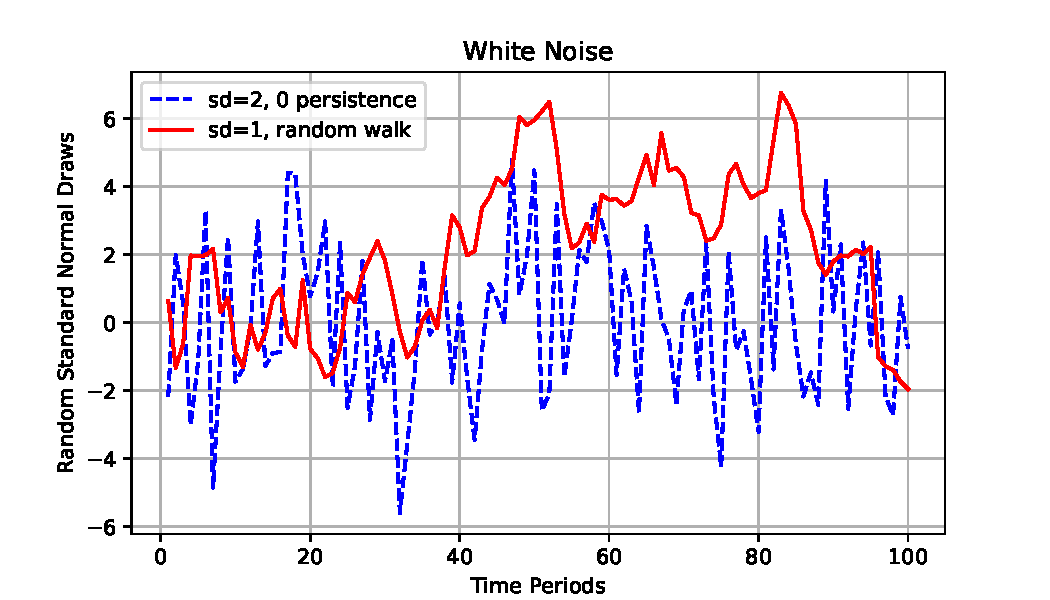
\includegraphics{A-Collection-of-Python-Examples_files/figure-latex/unnamed-chunk-13-1} \end{center}

\hypertarget{text-plot}{%
\subsection{Text Plot}\label{text-plot}}

\begin{quote}
Go back to \href{http://fanwangecon.github.io/}{fan}'s \href{https://fanwangecon.github.io/pyfan/}{Python Code Examples} Repository (\href{https://fanwangecon.github.io/pyfan/bookdown}{bookdown site}).
\end{quote}

\hypertarget{plot-text}{%
\subsubsection{Plot Text}\label{plot-text}}

Plot Text as Image. \href{https://matplotlib.org/3.1.1/gallery/pyplots/text_layout.html\#sphx-glr-gallery-pyplots-text-layout-py}{Create text with different alignment and rotation.}

\begin{Shaded}
\begin{Highlighting}[]
\CommentTok{# Import Packages}
\ImportTok{import}\NormalTok{ matplotlib.pyplot }\ImportTok{as}\NormalTok{ plt}
\ImportTok{import}\NormalTok{ textwrap}
\ImportTok{import}\NormalTok{ json}

\CommentTok{# Dict of String to String}
\NormalTok{dc_path }\OperatorTok{=}\NormalTok{ \{}\StringTok{'C:}\CharTok{\textbackslash{}\textbackslash{}}\StringTok{Users}\CharTok{\textbackslash{}\textbackslash{}}\StringTok{fan}\CharTok{\textbackslash{}\textbackslash{}}\StringTok{Documents}\CharTok{\textbackslash{}\textbackslash{}}\StringTok{Dropbox (UH-ECON)}\CharTok{\textbackslash{}\textbackslash{}}\StringTok{repos}\CharTok{\textbackslash{}\textbackslash{}}\StringTok{Tex4Econ}\CharTok{\textbackslash{}\textbackslash{}}\StringTok{'}
           \StringTok{'_other}\CharTok{\textbackslash{}\textbackslash{}}\StringTok{equation}\CharTok{\textbackslash{}\textbackslash{}}\StringTok{cases.tex'}\NormalTok{:}
               \StringTok{'C:/Users/fan/Documents/cases.pdf'}\NormalTok{,}
           \StringTok{'C:}\CharTok{\textbackslash{}\textbackslash{}}\StringTok{Users}\CharTok{\textbackslash{}\textbackslash{}}\StringTok{fan}\CharTok{\textbackslash{}\textbackslash{}}\StringTok{Documents}\CharTok{\textbackslash{}\textbackslash{}}\StringTok{Dropbox (UH-ECON)}\CharTok{\textbackslash{}\textbackslash{}}\StringTok{repos}\CharTok{\textbackslash{}\textbackslash{}}\StringTok{Tex4Econ}\CharTok{\textbackslash{}\textbackslash{}}\StringTok{'}
           \StringTok{'_other}\CharTok{\textbackslash{}\textbackslash{}}\StringTok{symbols}\CharTok{\textbackslash{}\textbackslash{}}\StringTok{fs_symbols.tex'}\NormalTok{:}
               \StringTok{'C:/Users/fan/Documents/fs_symbols.pdf'}\NormalTok{\}}
\NormalTok{st_dc_path }\OperatorTok{=}\NormalTok{ textwrap.fill(json.dumps(dc_path), width }\OperatorTok{=} \DecValTok{70}\NormalTok{)}

\CommentTok{# Start Plot}
\NormalTok{fig, ax }\OperatorTok{=}\NormalTok{ plt.subplots()}

\CommentTok{# Text Plot}
\NormalTok{ax.text(}\FloatTok{0.5}\NormalTok{, }\FloatTok{0.5}\NormalTok{, st_dc_path,}
\NormalTok{        horizontalalignment}\OperatorTok{=}\StringTok{'center'}\NormalTok{,}
\NormalTok{        verticalalignment}\OperatorTok{=}\StringTok{'center'}\NormalTok{,}
\NormalTok{        fontsize}\OperatorTok{=}\DecValTok{14}\NormalTok{, color}\OperatorTok{=}\StringTok{'black'}\NormalTok{,}
\NormalTok{        transform}\OperatorTok{=}\NormalTok{ax.transAxes)}

\CommentTok{# Labeling}
\end{Highlighting}
\end{Shaded}

\begin{verbatim}
## Text(0.5, 0.5, '{"C:\\\\Users\\\\fan\\\\Documents\\\\Dropbox (UH-\nECON)\\\\repos\\\\Tex4Econ\\\\_other\\\\equation\\\\cases.tex":\n"C:/Users/fan/Documents/cases.pdf",\n"C:\\\\Users\\\\fan\\\\Documents\\\\Dropbox (UH-\nECON)\\\\repos\\\\Tex4Econ\\\\_other\\\\symbols\\\\fs_symbols.tex":\n"C:/Users/fan/Documents/fs_symbols.pdf"}')
\end{verbatim}

\begin{Shaded}
\begin{Highlighting}[]
\NormalTok{ax.set_axis_off()}
\NormalTok{plt.show()}
\end{Highlighting}
\end{Shaded}

\begin{center}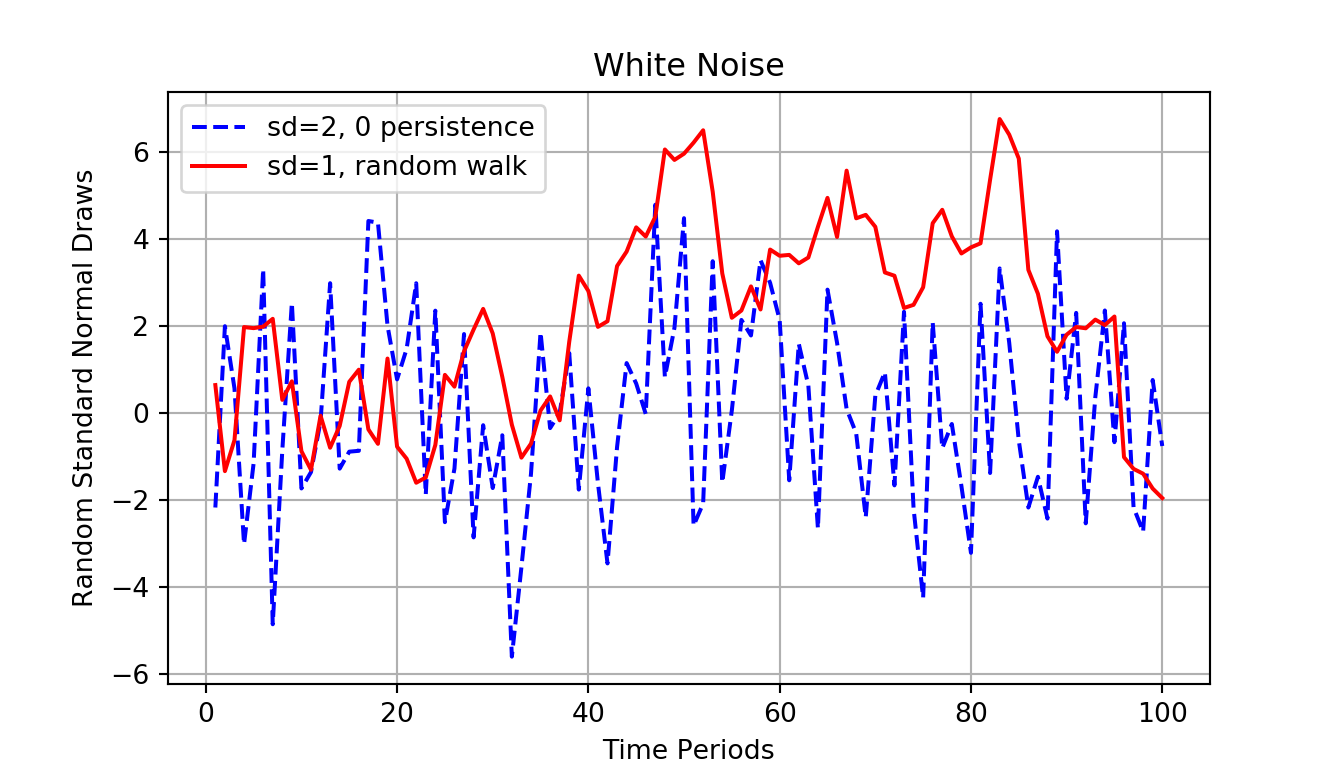
\includegraphics{A-Collection-of-Python-Examples_files/figure-latex/unnamed-chunk-15-1} \end{center}

\hypertarget{get-data}{%
\chapter{Get Data}\label{get-data}}

\hypertarget{environmental-data}{%
\section{Environmental Data}\label{environmental-data}}

\hypertarget{ecmwf-era5-data}{%
\subsection{ECMWF ERA5 Data}\label{ecmwf-era5-data}}

\begin{quote}
Go back to \href{http://fanwangecon.github.io/}{fan}'s \href{https://fanwangecon.github.io/pyfan/}{Python Code Examples} Repository (\href{https://fanwangecon.github.io/pyfan/bookdown}{bookdown site}).
\end{quote}

\hypertarget{basic-conda-setup}{%
\subsubsection{Basic Conda Setup}\label{basic-conda-setup}}

\begin{enumerate}
\def\labelenumi{\arabic{enumi}.}
\item
  Download \href{https://www.anaconda.com/products/individual}{Anaconda} for Python 3. For more involved conda instructions see \href{https://fanwangecon.github.io/Tex4Econ/nontex/install/windows/fn_installations.html}{here}
\item
  Open up \emph{anaconda prompt} with admin rights (right click choose as admin).

\begin{Shaded}
\begin{Highlighting}[]
\CommentTok{# Inside anaconda prompt}
\ExtensionTok{where}\NormalTok{ python}
\ExtensionTok{where}\NormalTok{ anaconda}
\CommentTok{# C:/ProgramData/Anaconda3/Scripts/anaconda.exe}
\CommentTok{# C:/ProgramData/Anaconda3/python.exe}
\end{Highlighting}
\end{Shaded}
\item
  Add to Path
\item
  Install cdsapi and eccodes

\begin{Shaded}
\begin{Highlighting}[]
\ExtensionTok{conda}\NormalTok{ config --add channels conda-forge}
\ExtensionTok{conda}\NormalTok{ install -c conda-forge eccodes -y}
\end{Highlighting}
\end{Shaded}
\end{enumerate}

\hypertarget{account-registration}{%
\subsubsection{Account Registration}\label{account-registration}}

\begin{enumerate}
\def\labelenumi{\arabic{enumi}.}
\item
  Register for an \href{cds.climate.copernicus.eu}{account}
\item
  \href{https://cds.climate.copernicus.eu/cdsapp/\#!/terms/licence-to-use-copernicus-products}{Agree to Licence}
\item
  Go to your CDS user page copy the url and key: \href{https://cds.climate.copernicus.eu/user}{Get url and key}

  \begin{itemize}
  \tightlist
  \item
    this has UID, 4XXXX, and API KEY, 4XXXfXXX-XXXf-4XXX-9XXX-7XXXebXXfdXX
  \item
    together they should look like: 4XXXX:4XXXfXXX-XXXf-4XXX-9XXX-7XXXebXXfdXX
  \end{itemize}
\item
  Open up an editor (notepad++ for example), create an empty file, paste the url and your UID:APIKEY into the file as below. Save file as: \emph{C:/Users/fan/.cdsapirc}. Under user root, as \emph{.cdsapirc} file. Note \emph{.cdsapirc} is the file name, you are saving that under the directory \emph{C:/Users/fan/}.

\begin{Shaded}
\begin{Highlighting}[]
\ExtensionTok{url}\NormalTok{: https://cds.climate.copernicus.eu/api/v2}
\ExtensionTok{key}\NormalTok{: 4XXXX:4XXXfXXX-XXXf-4XXX-9XXX-7XXXebXXfdXX}
\end{Highlighting}
\end{Shaded}
\end{enumerate}

\hypertarget{run-api-request-via-jupyter-notebook}{%
\subsubsection{Run API Request via Jupyter Notebook}\label{run-api-request-via-jupyter-notebook}}

\begin{enumerate}
\def\labelenumi{\arabic{enumi}.}
\item
  open up Jupyter Notebook (this opens up a browser page)

  \begin{itemize}
  \tightlist
  \item
    cd ``C:/Users/fan/Downloads''
  \item
    jupyter notebook
  \end{itemize}
\item
  create a new \emph{python3} file somewhere you like
\item
  name the file \emph{cdstest} (saved as ipynb file)
\item
  paste the code below inside the \emph{ipynb} file you opened (modify \emph{spt\_root}):

\begin{Shaded}
\begin{Highlighting}[]
\ImportTok{import}\NormalTok{ cdsapi}
\ImportTok{import}\NormalTok{ urllib.request}
\CommentTok{# download folder}
\NormalTok{spt_root }\OperatorTok{=} \StringTok{"C:/Users/fan/downloads/_data/"}
\NormalTok{spn_dl_test_grib }\OperatorTok{=}\NormalTok{ spt_root }\OperatorTok{+} \StringTok{"test_china_temp.grib"}
\CommentTok{# request}
\NormalTok{c }\OperatorTok{=}\NormalTok{ cdsapi.Client()}
\NormalTok{res }\OperatorTok{=}\NormalTok{ c.retrieve(}\StringTok{"reanalysis-era5-pressure-levels"}\NormalTok{,}
\NormalTok{  \{}
    \StringTok{'product_type'}\NormalTok{: }\StringTok{'reanalysis'}\NormalTok{,}
    \StringTok{'variable'}\NormalTok{: }\StringTok{'temperature'}\NormalTok{,}
    \StringTok{'pressure_level'}\NormalTok{: }\StringTok{'1000'}\NormalTok{,}
    \StringTok{'year'}\NormalTok{: }\StringTok{'2008'}\NormalTok{,}
    \StringTok{'month'}\NormalTok{: }\StringTok{'01'}\NormalTok{,}
    \StringTok{'day'}\NormalTok{: }\StringTok{'01'}\NormalTok{,}
    \StringTok{'time'}\NormalTok{: }\StringTok{'12:00'}\NormalTok{,}
    \StringTok{'format'}\NormalTok{: }\StringTok{'netcdf'}\NormalTok{,}
    \StringTok{'area'}\NormalTok{          : [}\FloatTok{53.31}\NormalTok{, }\DecValTok{73}\NormalTok{, }\FloatTok{4.15}\NormalTok{, }\DecValTok{135}\NormalTok{],}
    \StringTok{'grid'}\NormalTok{          : [}\FloatTok{1.0}\NormalTok{, }\FloatTok{1.0}\NormalTok{],}
    \StringTok{"format"}\NormalTok{: }\StringTok{"grib"}
\NormalTok{  \},}
\NormalTok{  spn_dl_test_grib}
\NormalTok{)}
\CommentTok{# show results}
\BuiltInTok{print}\NormalTok{(}\StringTok{'print results'}\NormalTok{)}
\BuiltInTok{print}\NormalTok{(res)}
\BuiltInTok{print}\NormalTok{(}\BuiltInTok{type}\NormalTok{(res))}
\end{Highlighting}
\end{Shaded}
\item
  click run
\end{enumerate}

\hypertarget{run-api-request-via-ipython}{%
\subsubsection{Run API request via Ipython}\label{run-api-request-via-ipython}}

\begin{enumerate}
\def\labelenumi{\arabic{enumi}.}
\tightlist
\item
  In Anaconda Prompt: \emph{ipython}
\item
  Open a file in notepad++ or elsewhere, copy the code above over and edit the spt\_root to reflect your directories
\item
  Select the entire code in the notepad++ page, and copy all lines
\item
  Now inside ipython, type percentage and paste: \%paste
\item
  This should run the file above and save the grib file in the folder you specified with the name you specified.
\end{enumerate}

\hypertarget{convert-crib-data-to-csv}{%
\subsubsection{Convert CRIB data to CSV}\label{convert-crib-data-to-csv}}

\begin{enumerate}
\def\labelenumi{\arabic{enumi}.}
\item
  inside conda prompt cd into the folder where you downloaded the grib file
\item
  \emph{grib\_ls} shows what is in the grib file
\item
  \emph{grib\_get\_data} translates grib to csv

\begin{Shaded}
\begin{Highlighting}[]
\BuiltInTok{cd} \StringTok{"C:/Users/fan/downloads/_data/"}
\ExtensionTok{grib_ls}\NormalTok{ test_china_temp.grib}
\ExtensionTok{grib_get_data}\NormalTok{ test_china_temp.grib }\OperatorTok{>}\NormalTok{ test_china_temp_raw.csv}
\end{Highlighting}
\end{Shaded}
\end{enumerate}

\hypertarget{more-advanced-download-setup-and-instructions}{%
\subsubsection{More Advanced Download Setup and Instructions}\label{more-advanced-download-setup-and-instructions}}

\hypertarget{conda-enviornment-and-installation}{%
\paragraph{Conda Enviornment and Installation}\label{conda-enviornment-and-installation}}

In conda, set up a conda environment for downloading ECMWF data using the ECMWF API. (\href{https://fanwangecon.github.io/Tex4Econ/nontex/install/windows/fn_installations.html}{Conda Set-up})

\begin{Shaded}
\begin{Highlighting}[]
\CommentTok{# Set up}
\ExtensionTok{conda}\NormalTok{ deactivate}
\ExtensionTok{conda}\NormalTok{ list env}
\ExtensionTok{conda}\NormalTok{ env remove -n wk_ecmwf}
\ExtensionTok{conda}\NormalTok{ create -n wk_ecmwf -y}
\ExtensionTok{conda}\NormalTok{ activate wk_ecmwf}

\CommentTok{# Add conda-forge to channel in env}
\ExtensionTok{conda}\NormalTok{ config --env --add channels conda-forge}
\ExtensionTok{conda}\NormalTok{ config --get channels}
\ExtensionTok{conda}\NormalTok{ config --get channels --env}

\CommentTok{# Install}
\ExtensionTok{conda}\NormalTok{ install cdsapi -y}
\ExtensionTok{conda}\NormalTok{ install -c conda-forge eccodes -y}
\end{Highlighting}
\end{Shaded}

This creates the conda env that we are using here for python.

\hypertarget{config-file-.cdsapirc}{%
\paragraph{Config File .cdsapirc}\label{config-file-.cdsapirc}}

Open up the \emph{cdsapirc}, create new if does note exist. Below, open up the file and save the text. See \href{https://fanwangecon.github.io/pyfan/vig/support/inout/htmlpdfr/fp_files.html}{Python Reading and Writing to File Examples}.

First, get the text for the config file:

\begin{Shaded}
\begin{Highlighting}[]
\NormalTok{stf_cds_cdsapirc }\OperatorTok{=} \StringTok{"""\textbackslash{}}
\StringTok{url: https://cds.climate.copernicus.eu/api/v2}
\StringTok{key: 4XXXX:4XXXfXXX-XXXf-4XXX-9XXX-7XXXebXXfdXX\textbackslash{}}
\StringTok{"""}
\BuiltInTok{print}\NormalTok{(stf_cds_cdsapirc)}
\end{Highlighting}
\end{Shaded}

Second save text to file:

\begin{Shaded}
\begin{Highlighting}[]
\CommentTok{# Relative file name}
\NormalTok{spt_file_cds }\OperatorTok{=} \StringTok{"C:/Users/fan/"}
\NormalTok{snm_file_cds }\OperatorTok{=} \StringTok{".cdsapirc"}
\NormalTok{spn_file_cds }\OperatorTok{=}\NormalTok{ spt_file_cds }\OperatorTok{+}\NormalTok{ snm_file_cds}
\CommentTok{# Open new file}
\NormalTok{fl_cdsapirc_contents }\OperatorTok{=} \BuiltInTok{open}\NormalTok{(spn_file_cds, }\StringTok{'w'}\NormalTok{)}
\CommentTok{# Write to File}
\NormalTok{fl_cdsapirc_contents.write(stf_cds_cdsapirc)}
\CommentTok{# Close}
\NormalTok{fl_cdsapirc_contents.close()}
\end{Highlighting}
\end{Shaded}

\begin{Shaded}
\begin{Highlighting}[]
\CommentTok{# Open the config file to check}
\ExtensionTok{code} \StringTok{"C:/Users/fan/.cdsapirc"}
\end{Highlighting}
\end{Shaded}

\hypertarget{generate-api-requests}{%
\subsubsection{Generate API Requests}\label{generate-api-requests}}

Go to the sites below, choose download data, pick what is needed, and then select \emph{Show API request} at the bottom of page:

\textbf{ERA5 pressure levels from 1979 to present}

\begin{itemize}
\tightlist
\item
  \href{https://cds.climate.copernicus.eu/cdsapp\#!/dataset/reanalysis-era5-pressure-levels}{ERA5 hourly pressure}
\item
  \href{https://cds.climate.copernicus.eu/cdsapp\#!/dataset/reanalysis-era5-pressure-levels-monthly-means}{ERA5 monthly pressure}
\end{itemize}

\textbf{ERA5 single levels from 1979 to present}

\begin{itemize}
\tightlist
\item
  \href{https://cds.climate.copernicus.eu/cdsapp\#!/dataset/reanalysis-era5-single-levels}{ERA5 hourly pressure}
\item
  \href{https://cds.climate.copernicus.eu/cdsapp\#!/dataset/reanalysis-era5-single-levels-monthly-means}{ERA5 monthly pressure}
\end{itemize}

\hypertarget{api-request-china-temp-test}{%
\paragraph{API Request China Temp Test}\label{api-request-china-temp-test}}

API function is \href{https://github.com/ecmwf/cdsapi/blob/master/cdsapi/api.py}{here}.

Select based on China's area, some testing data and download grib file. The data is from 2008, Jan 1st, at 12 noon?

Open up Jupyter notebook: \emph{jupyter notebook}

\begin{Shaded}
\begin{Highlighting}[]
\CommentTok{# import module in conda env wk_ecmwf}
\ImportTok{import}\NormalTok{ cdsapi}
\ImportTok{import}\NormalTok{ urllib.request}

\CommentTok{# download folder}
\NormalTok{spt_root }\OperatorTok{=} \StringTok{"C:/Users/fan/pyfan/vig/getdata/envir/"}
\NormalTok{spn_dl_test_grib }\OperatorTok{=}\NormalTok{ spt_root }\OperatorTok{+} \StringTok{"_data/test/test_china_temp.grib"}

\CommentTok{# request}
\NormalTok{c }\OperatorTok{=}\NormalTok{ cdsapi.Client()}
\NormalTok{res }\OperatorTok{=}\NormalTok{ c.retrieve(}\StringTok{"reanalysis-era5-pressure-levels"}\NormalTok{,}
\NormalTok{  \{}
    \StringTok{'product_type'}\NormalTok{: }\StringTok{'reanalysis'}\NormalTok{,}
    \StringTok{'variable'}\NormalTok{: }\StringTok{'temperature'}\NormalTok{,}
    \StringTok{'pressure_level'}\NormalTok{: }\StringTok{'1000'}\NormalTok{,}
    \StringTok{'year'}\NormalTok{: }\StringTok{'2008'}\NormalTok{,}
    \StringTok{'month'}\NormalTok{: }\StringTok{'01'}\NormalTok{,}
    \StringTok{'day'}\NormalTok{: }\StringTok{'01'}\NormalTok{,}
    \StringTok{'time'}\NormalTok{: }\StringTok{'12:00'}\NormalTok{,}
    \StringTok{'format'}\NormalTok{: }\StringTok{'netcdf'}\NormalTok{,}
    \StringTok{'area'}\NormalTok{          : [}\FloatTok{53.31}\NormalTok{, }\DecValTok{73}\NormalTok{, }\FloatTok{4.15}\NormalTok{, }\DecValTok{135}\NormalTok{],}
    \StringTok{'grid'}\NormalTok{          : [}\FloatTok{1.0}\NormalTok{, }\FloatTok{1.0}\NormalTok{],}
    \StringTok{"format"}\NormalTok{: }\StringTok{"grib"}
\NormalTok{  \},}
\NormalTok{  spn_dl_test_grib}
\NormalTok{)}
\CommentTok{# show results}
\BuiltInTok{print}\NormalTok{(}\StringTok{'print results'}\NormalTok{)}
\BuiltInTok{print}\NormalTok{(res)}
\BuiltInTok{print}\NormalTok{(}\BuiltInTok{type}\NormalTok{(res))}

\CommentTok{# download}
\CommentTok{# response = urllib.request.urlopen('http://www.example.com/')}
\CommentTok{# html = response.read()}
\end{Highlighting}
\end{Shaded}

\begin{quote}
2020-06-17 23:51:35,107 INFO Welcome to the CDS
2020-06-17 23:51:35,107 INFO Sending request to \url{https://cds.climate.copernicus.eu/api/v2/resources/reanalysis-era5-pressure-levels}
2020-06-17 23:51:36,441 INFO Request is queued
2020-06-17 23:51:39,183 INFO Request is running
2020-06-17 23:51:45,059 INFO Request is completed
2020-06-17 23:51:45,060 INFO Downloading \textgreater{} \url{http://136.156.133.25/cache-compute-0008/cache/data2/adaptor.mars.internal-1592455900.8655114-11162-11-68e1ea23-8985-4926-95e6-9f181cc7792}\textgreater{} 7.grib to C:/Users/fan/pyfan/vig/getdata/envir/\_data/test/test\_china\_temp.grib (6.3K)
2020-06-17 23:51:45,441 INFO Download rate 16.6K/s
print results
Result(content\_length=6480,content\_type=application/x-grib,location=\url{http://136.156.133.25/cache-compute-0008/cache/data2/adaptor.mars.inte}\textgreater{} rnal-1592455900.8655114-11162-11-68e1ea23-8985-4926-95e6-9f181cc77927.grib)
\textless class `cdsapi.api.Result'\textgreater{}
\end{quote}

Convert grib to raw csv, open up command line:

\begin{Shaded}
\begin{Highlighting}[]
\BuiltInTok{cd} \StringTok{"C:/Users/fan/pyfan/vig/getdata/envir/_data/test/"}
\ExtensionTok{grib_ls}\NormalTok{ test_china_temp.grib}
\ExtensionTok{grib_get_data}\NormalTok{ test_china_temp.grib }\OperatorTok{>}\NormalTok{ test_china_temp_raw.csv}
\end{Highlighting}
\end{Shaded}

Format the CSV file (is not comma separated)

\begin{Shaded}
\begin{Highlighting}[]
\NormalTok{spt_root }\OperatorTok{=} \StringTok{"C:/Users/fan/pyfan/vig/getdata/envir/_data/test/"}
\NormalTok{spn_csv_raw }\OperatorTok{=}\NormalTok{ spt_root }\OperatorTok{+} \StringTok{"test_china_temp_raw.csv"}
\NormalTok{spn_csv_edi }\OperatorTok{=}\NormalTok{ spt_root }\OperatorTok{+} \StringTok{"test_china_temp.csv"}

\ControlFlowTok{with} \BuiltInTok{open}\NormalTok{(spn_csv_raw, }\StringTok{'r'}\NormalTok{) }\ImportTok{as}\NormalTok{ f_in, }\BuiltInTok{open}\NormalTok{(spn_csv_edi, }\StringTok{'w'}\NormalTok{) }\ImportTok{as}\NormalTok{ f_out:}
\NormalTok{    f_out.write(}\BuiltInTok{next}\NormalTok{(f_in))}
\NormalTok{    [f_out.write(}\StringTok{','}\NormalTok{.join(line.split()) }\OperatorTok{+} \StringTok{'}\CharTok{\textbackslash{}n}\StringTok{'}\NormalTok{) }\ControlFlowTok{for}\NormalTok{ line }\KeywordTok{in}\NormalTok{ f_in]}
\end{Highlighting}
\end{Shaded}

Show CSV results:

\begin{Shaded}
\begin{Highlighting}[]
\CommentTok{# Path and Read}
\NormalTok{spt_root =}\StringTok{ "C:/Users/fan/pyfan/vig/getdata/envir/"}
\NormalTok{spn_dl_test_csv =}\StringTok{ }\KeywordTok{paste0}\NormalTok{(spt_root, }\StringTok{"_data/test/test_china_temp.csv"}\NormalTok{)}
\NormalTok{china_weather_data <-}\StringTok{ }\KeywordTok{read.csv}\NormalTok{(spn_dl_test_csv)}

\CommentTok{# Top 50 rows}
\KeywordTok{kable}\NormalTok{(}\KeywordTok{head}\NormalTok{(china_weather_data, }\DecValTok{50}\NormalTok{),}
      \DataTypeTok{caption=}\StringTok{"Chinese Long and Lat, Temperature Pressure, 2008 Jan 1st at 12 noon?"}\NormalTok{) }\OperatorTok
\StringTok{  }\KeywordTok{kable_styling_fc}\NormalTok{()}
\end{Highlighting}
\end{Shaded}

\begin{table}[!h]

\caption{\label{tab:unnamed-chunk-29}Chinese Long and Lat, Temperature Pressure, 2008 Jan 1st at 12 noon?}
\centering
\begin{tabular}[t]{r|r|r}
\hline
Latitude & Longitude & Value\\
\hline
\rowcolor{gray!6}  53.15 & 73 & 260.6515\\
\hline
53.15 & 74 & 259.9796\\
\hline
\rowcolor{gray!6}  53.15 & 75 & 259.2227\\
\hline
53.15 & 76 & 258.5929\\
\hline
\rowcolor{gray!6}  53.15 & 77 & 258.2765\\
\hline
53.15 & 78 & 258.0636\\
\hline
\rowcolor{gray!6}  53.15 & 79 & 258.0069\\
\hline
53.15 & 80 & 257.7267\\
\hline
\rowcolor{gray!6}  53.15 & 81 & 258.8370\\
\hline
53.15 & 82 & 260.9239\\
\hline
\rowcolor{gray!6}  53.15 & 83 & 262.5440\\
\hline
53.15 & 84 & 263.9083\\
\hline
\rowcolor{gray!6}  53.15 & 85 & 264.8976\\
\hline
53.15 & 86 & 264.6729\\
\hline
\rowcolor{gray!6}  53.15 & 87 & 264.1827\\
\hline
53.15 & 88 & 265.0587\\
\hline
\rowcolor{gray!6}  53.15 & 89 & 264.9425\\
\hline
53.15 & 90 & 266.2960\\
\hline
\rowcolor{gray!6}  53.15 & 91 & 269.0958\\
\hline
53.15 & 92 & 270.3165\\
\hline
\rowcolor{gray!6}  53.15 & 93 & 269.0030\\
\hline
53.15 & 94 & 268.4210\\
\hline
\rowcolor{gray!6}  53.15 & 95 & 264.9591\\
\hline
53.15 & 96 & 261.9249\\
\hline
\rowcolor{gray!6}  53.15 & 97 & 264.5304\\
\hline
53.15 & 98 & 265.3995\\
\hline
\rowcolor{gray!6}  53.15 & 99 & 268.2374\\
\hline
53.15 & 100 & 269.9444\\
\hline
\rowcolor{gray!6}  53.15 & 101 & 272.6202\\
\hline
53.15 & 102 & 270.6798\\
\hline
\rowcolor{gray!6}  53.15 & 103 & 270.0919\\
\hline
53.15 & 104 & 269.6876\\
\hline
\rowcolor{gray!6}  53.15 & 105 & 271.4718\\
\hline
53.15 & 106 & 271.2403\\
\hline
\rowcolor{gray!6}  53.15 & 107 & 271.1163\\
\hline
53.15 & 108 & 269.3849\\
\hline
\rowcolor{gray!6}  53.15 & 109 & 270.7247\\
\hline
53.15 & 110 & 269.6388\\
\hline
\rowcolor{gray!6}  53.15 & 111 & 268.6622\\
\hline
53.15 & 112 & 267.6036\\
\hline
\rowcolor{gray!6}  53.15 & 113 & 267.4796\\
\hline
53.15 & 114 & 266.6983\\
\hline
\rowcolor{gray!6}  53.15 & 115 & 266.2911\\
\hline
53.15 & 116 & 266.5880\\
\hline
\rowcolor{gray!6}  53.15 & 117 & 265.4513\\
\hline
53.15 & 118 & 264.4630\\
\hline
\rowcolor{gray!6}  53.15 & 119 & 260.6183\\
\hline
53.15 & 120 & 259.3018\\
\hline
\rowcolor{gray!6}  53.15 & 121 & 258.4161\\
\hline
53.15 & 122 & 258.8429\\
\hline
\end{tabular}
\end{table}

``ERA5 is a comprehensive reanalysis, from 1979 (soon to be backdated to 1950) to near real time, which assimilates as many observations as possible in the upper air and near surface. The ERA5 atmospheric model is coupled with a land surface model and a wave model.''

\begin{enumerate}
\def\labelenumi{\arabic{enumi}.}
\tightlist
\item
  Register for an \href{cds.climate.copernicus.eu}{account}
\item
  \href{https://cds.climate.copernicus.eu/cdsapp/\#!/terms/licence-to-use-copernicus-products}{Agree to Licence}
\end{enumerate}

\hypertarget{learning}{%
\subsubsection{Learning}\label{learning}}

\hypertarget{terminologies}{%
\paragraph{Terminologies}\label{terminologies}}

\textbf{Links}:

\begin{itemize}
\tightlist
\item
  \href{https://cds.climate.copernicus.eu/live/queue}{status of the CDS queue}.
\end{itemize}

\textbf{Terminologies}:

\begin{itemize}
\tightlist
\item
  \href{}{single level parameters}
\end{itemize}

\hypertarget{single-level-parameters}{%
\paragraph{Single Level Parameters}\label{single-level-parameters}}

\href{https://confluence.ecmwf.int/display/CKB/ERA5?src=breadcrumbs-parent}{ERA5 Variables}?

\begin{enumerate}
\def\labelenumi{\arabic{enumi}.}
\tightlist
\item
  \href{https://confluence.ecmwf.int/pages/viewpage.action?pageId=82870405\#ERA5:datadocumentation-Table1}{Table 1: surface and single level parameters: invariants}
\item
  \href{https://confluence.ecmwf.int/pages/viewpage.action?pageId=82870405\#ERA5:datadocumentation-Table9}{Table 9: pressure level parameters: instantaneous}
\end{enumerate}

\begin{itemize}
\tightlist
\item
  Temperature
\end{itemize}

\href{https://confluence.ecmwf.int/display/CKB/How+to+download+ERA5}{ER5 Data Download Instructions}.

\hypertarget{download-unzip-convert-to-combined-csv}{%
\subsubsection{Download, Unzip, Convert to combined CSV}\label{download-unzip-convert-to-combined-csv}}

The data downloaded from CDS climate could become very large in size. We want to process parts of the data one part at a time, summarize and aggregate over each part, and generate a file output file with aggregate statistics over the entire time period of interest.

This code below accompalishes the following tasks:

\begin{enumerate}
\def\labelenumi{\arabic{enumi}.}
\tightlist
\item
  download data from derived-utci-historical as ZIP
\item
  unzip
\item
  convert \emph{nc} files to \emph{csv} files
\item
  individual csv files are half year groups
\end{enumerate}

Parameter Control for the code below:

\begin{enumerate}
\def\labelenumi{\arabic{enumi}.}
\tightlist
\item
  \emph{spt\_root}: root folder where everything will be at
\item
  \emph{spth\_conda\_env}: the conda virtual environment python path, eccodes and cdsapi packages are installed in the conda virtual environment. In the example below, the first env is: wk\_ecmwf
\item
  \emph{st\_nc\_prefix}: the downloaded individual nc files have dates and prefix before and after the date string in the nc file names. This is the string before that.
\item
  \emph{st\_nc\_suffix}: see (3), this is the suffix
\item
  \emph{ar\_years}: array of years to download and aggregate over
\item
  \emph{ar\_months\_g1}: months to download in first half year
\item
  \emph{ar\_months\_g2}: months to download in second half year
\end{enumerate}

\begin{Shaded}
\begin{Highlighting}[]
\CommentTok{#################################################}
\CommentTok{# ------------ Parameters}
\CommentTok{#################################################}

\CommentTok{# Where to store everything}
\NormalTok{spt_root <-}\StringTok{ "C:/Users/fan/Downloads/_data/"}
\NormalTok{spth_conda_env <-}\StringTok{ "C:/ProgramData/Anaconda3/envs/wk_ecmwf/python.exe"}
\CommentTok{# nc name prefix}
\NormalTok{st_nc_prefix <-}\StringTok{ "ECMWF_utci_"}
\NormalTok{st_nc_suffix <-}\StringTok{ "_v1.0_con.nc"}
\CommentTok{# Years list}
\CommentTok{# ar_years <- 2001:2019}
\NormalTok{ar_years <-}\StringTok{ }\KeywordTok{c}\NormalTok{(}\DecValTok{2005}\NormalTok{, }\DecValTok{2015}\NormalTok{)}
\CommentTok{# ar_months_g1 <- c('01','02','03','04','05','06')}
\NormalTok{ar_months_g1 <-}\StringTok{ }\KeywordTok{c}\NormalTok{(}\StringTok{'01'}\NormalTok{, }\StringTok{'03'}\NormalTok{)}
\CommentTok{# ar_months_g2 <- c('07','08','09','10','11','12')}
\NormalTok{ar_months_g2 <-}\StringTok{ }\KeywordTok{c}\NormalTok{(}\StringTok{'07'}\NormalTok{, }\StringTok{'09'}\NormalTok{)}


\CommentTok{# folder to download any nc zips to}
\NormalTok{nczippath <-}\StringTok{ }\NormalTok{spt_root}
\CommentTok{# we are changing the python api file with different requests stirngs and storing it here}
\NormalTok{pyapipath <-}\StringTok{ }\NormalTok{spt_root}
\CommentTok{# output directory for AGGREGATE CSV with all DATES from this search}
\NormalTok{csvpath <-}\StringTok{ }\NormalTok{spt_root}

\CommentTok{#################################################}
\CommentTok{# ------------ Packages}
\CommentTok{#################################################}

\KeywordTok{library}\NormalTok{(}\StringTok{"ncdf4"}\NormalTok{)}
\KeywordTok{library}\NormalTok{(}\StringTok{"chron"}\NormalTok{)}
\KeywordTok{library}\NormalTok{(}\StringTok{"lattice"}\NormalTok{)}
\KeywordTok{library}\NormalTok{(}\StringTok{"RColorBrewer"}\NormalTok{)}
\KeywordTok{library}\NormalTok{(}\StringTok{"stringr"}\NormalTok{)}
\KeywordTok{library}\NormalTok{(}\StringTok{"tibble"}\NormalTok{)}
\KeywordTok{library}\NormalTok{(}\StringTok{"dplyr"}\NormalTok{)}
\KeywordTok{Sys.setenv}\NormalTok{(}\DataTypeTok{RETICULATE_PYTHON =}\NormalTok{ spth_conda_env)}
\KeywordTok{library}\NormalTok{(}\StringTok{"reticulate"}\NormalTok{)}

\CommentTok{#################################################}
\CommentTok{# ------------ Define Loops}
\CommentTok{#################################################}
\ControlFlowTok{for}\NormalTok{ (it_yr }\ControlFlowTok{in}\NormalTok{ ar_years) \{}
  \ControlFlowTok{for}\NormalTok{ (it_mth_group }\ControlFlowTok{in} \KeywordTok{c}\NormalTok{(}\DecValTok{1}\NormalTok{,}\DecValTok{2}\NormalTok{)) \{}
    \ControlFlowTok{if}\NormalTok{(it_mth_group }\OperatorTok{==}\StringTok{ }\DecValTok{1}\NormalTok{) \{}
\NormalTok{      ar_months =}\StringTok{ }\NormalTok{ar_months_g1}
\NormalTok{    \}}
    \ControlFlowTok{if}\NormalTok{(it_mth_group }\OperatorTok{==}\StringTok{ }\DecValTok{2}\NormalTok{) \{}
\NormalTok{      ar_months =}\StringTok{ }\NormalTok{ar_months_g2}
\NormalTok{    \}}

    \CommentTok{#################################################}
    \CommentTok{# ------------ Define Python API Call}
    \CommentTok{#################################################}

    \CommentTok{# name of zip file}
\NormalTok{    nczipname <-}\StringTok{ "derived_utci_2010_2.zip"}
\NormalTok{    unzipfolder <-}\StringTok{ "derived_utci_2010_2"}

\NormalTok{    st_file <-}\StringTok{ }\KeywordTok{paste0}\NormalTok{(}\StringTok{"import cdsapi}
\StringTok{import urllib.request}
\StringTok{# download folder}
\StringTok{spt_root = '"}\NormalTok{, nczippath, }\StringTok{"'}
\StringTok{spn_dl_test_grib = spt_root + '"}\NormalTok{, nczipname, }\StringTok{"'}
\StringTok{# request}
\StringTok{c = cdsapi.Client()}
\StringTok{res = c.retrieve(}
\StringTok{    'derived-utci-historical',}
\StringTok{    \{}
\StringTok{        'format': 'zip',}
\StringTok{        'variable': 'Universal thermal climate index',}
\StringTok{        'product_type': 'Consolidated dataset',}
\StringTok{        'year': '"}\NormalTok{,it_yr, }\StringTok{"',}
\StringTok{        'month': [}
\StringTok{            "}\NormalTok{, }\KeywordTok{paste}\NormalTok{(}\StringTok{"'"}\NormalTok{, ar_months, }\StringTok{"'"}\NormalTok{, }\DataTypeTok{sep =} \StringTok{""}\NormalTok{, }\DataTypeTok{collapse =} \StringTok{", "}\NormalTok{), }\StringTok{"}
\StringTok{        ],}
\StringTok{        'day': [}
\StringTok{            '01','03'}
\StringTok{        ],}
\StringTok{        'area'  : [53.31, 73, 4.15, 135],}
\StringTok{        'grid'  : [0.25, 0.25],}
\StringTok{    \},}
\StringTok{    spn_dl_test_grib)}
\StringTok{# show results}
\StringTok{print('print results')}
\StringTok{print(res)}
\StringTok{print(type(res))"}\NormalTok{)}

    \CommentTok{# st_file = "print(1+1)"}

    \CommentTok{# Store Python Api File}
\NormalTok{    fl_test_tex <-}\StringTok{ }\KeywordTok{paste0}\NormalTok{(pyapipath, }\StringTok{"api.py"}\NormalTok{)}
\NormalTok{    fileConn <-}\StringTok{ }\KeywordTok{file}\NormalTok{(fl_test_tex)}
    \KeywordTok{writeLines}\NormalTok{(st_file, fileConn)}
    \KeywordTok{close}\NormalTok{(fileConn)}

    \CommentTok{#################################################}
    \CommentTok{# ------------ Run Python File}
    \CommentTok{#################################################}
    \CommentTok{# Set Path}
    \KeywordTok{setwd}\NormalTok{(pyapipath)}
    \CommentTok{# Run py file, api.py name just defined}
    \KeywordTok{use_python}\NormalTok{(spth_conda_env)}
    \KeywordTok{source_python}\NormalTok{(}\StringTok{'api.py'}\NormalTok{)}

    \CommentTok{#################################################}
    \CommentTok{# ------------ uNZIP}
    \CommentTok{#################################################}
\NormalTok{    spn_zip <-}\StringTok{ }\KeywordTok{paste0}\NormalTok{(nczippath, nczipname)}
\NormalTok{    spn_unzip_folder <-}\StringTok{ }\KeywordTok{paste0}\NormalTok{(nczippath, unzipfolder)}
    \KeywordTok{unzip}\NormalTok{(spn_zip, }\DataTypeTok{exdir=}\NormalTok{spn_unzip_folder)}

    \CommentTok{#################################################}
    \CommentTok{# ------------ Find All files}
    \CommentTok{#################################################}
    \CommentTok{# Get all files with nc suffix in folder}
\NormalTok{    ncpath <-}\StringTok{ }\KeywordTok{paste0}\NormalTok{(nczippath, unzipfolder)}
\NormalTok{    ls_sfls <-}\StringTok{ }\KeywordTok{list.files}\NormalTok{(}\DataTypeTok{path=}\NormalTok{ncpath, }\DataTypeTok{recursive=}\OtherTok{TRUE}\NormalTok{, }\DataTypeTok{pattern=}\StringTok{".nc"}\NormalTok{, }\DataTypeTok{full.names=}\NormalTok{T)}

    \CommentTok{#################################################}
    \CommentTok{# ------------ Combine individual NC files to JOINT Dataframe}
    \CommentTok{#################################################}
    \CommentTok{# List to gather dataframes}
\NormalTok{    ls_df <-}\StringTok{ }\KeywordTok{vector}\NormalTok{(}\DataTypeTok{mode =} \StringTok{"list"}\NormalTok{, }\DataTypeTok{length =} \KeywordTok{length}\NormalTok{(ls_sfls))}
    \CommentTok{# Loop over files and convert nc to csv}
\NormalTok{    it_df_ctr <-}\StringTok{ }\DecValTok{0}
    \ControlFlowTok{for}\NormalTok{ (spt_file }\ControlFlowTok{in}\NormalTok{ ls_sfls) \{}
\NormalTok{      it_df_ctr <-}\StringTok{ }\NormalTok{it_df_ctr }\OperatorTok{+}\StringTok{ }\DecValTok{1}

      \CommentTok{# Get file name without Path}
\NormalTok{      snm_file_date <-}\StringTok{ }\KeywordTok{sub}\NormalTok{(}\KeywordTok{paste0}\NormalTok{(}\StringTok{'}\CharTok{\textbackslash{}\textbackslash{}}\StringTok{'}\NormalTok{,st_nc_suffix,}\StringTok{'$'}\NormalTok{), }\StringTok{''}\NormalTok{, }\KeywordTok{basename}\NormalTok{(spt_file))}
\NormalTok{      snm_file_date <-}\StringTok{ }\KeywordTok{sub}\NormalTok{(st_nc_prefix, }\StringTok{''}\NormalTok{, }\KeywordTok{basename}\NormalTok{(snm_file_date))}

      \CommentTok{# Dates Start and End: list.files is auto sorted in ascending order}
      \ControlFlowTok{if}\NormalTok{ (it_df_ctr }\OperatorTok{==}\StringTok{ }\DecValTok{1}\NormalTok{) \{}
\NormalTok{        snm_start_date <-}\StringTok{ }\NormalTok{snm_file_date}
\NormalTok{      \}}
      \ControlFlowTok{else}\NormalTok{ \{}
        \CommentTok{# this will give the final date}
\NormalTok{        snm_end_date <-}\StringTok{ }\NormalTok{snm_file_date}
\NormalTok{      \}}

      \CommentTok{# Given this structure: ECMWF_utci_20100702_v1.0_con, sub out prefix and suffix}
      \KeywordTok{print}\NormalTok{(spt_file)}
\NormalTok{      ncin <-}\StringTok{ }\KeywordTok{nc_open}\NormalTok{(spt_file)}

\NormalTok{      nchist <-}\StringTok{ }\KeywordTok{ncatt_get}\NormalTok{(ncin, }\DecValTok{0}\NormalTok{, }\StringTok{"history"}\NormalTok{)}

      \CommentTok{# not using this missing value flag at the moment}
\NormalTok{      missingval <-}\StringTok{ }\KeywordTok{str_match}\NormalTok{(nchist}\OperatorTok{$}\NormalTok{value, }\StringTok{"setmisstoc,}\CharTok{\textbackslash{}\textbackslash{}}\StringTok{s*(.*?)}\CharTok{\textbackslash{}\textbackslash{}}\StringTok{s* "}\NormalTok{)[,}\DecValTok{2}\NormalTok{]}
\NormalTok{      missingval <-}\StringTok{ }\KeywordTok{as.numeric}\NormalTok{(missingval)}

\NormalTok{      lon <-}\StringTok{ }\KeywordTok{ncvar_get}\NormalTok{(ncin, }\StringTok{"lon"}\NormalTok{)}
\NormalTok{      lat <-}\StringTok{ }\KeywordTok{ncvar_get}\NormalTok{(ncin, }\StringTok{"lat"}\NormalTok{)}
\NormalTok{      tim <-}\StringTok{ }\KeywordTok{ncvar_get}\NormalTok{(ncin, }\StringTok{"time"}\NormalTok{)}
\NormalTok{      tunits <-}\StringTok{ }\KeywordTok{ncatt_get}\NormalTok{(ncin, }\StringTok{"time"}\NormalTok{, }\StringTok{"units"}\NormalTok{)}

\NormalTok{      nlon <-}\StringTok{ }\KeywordTok{dim}\NormalTok{(lon)}
\NormalTok{      nlat <-}\StringTok{ }\KeywordTok{dim}\NormalTok{(lat)}
\NormalTok{      ntim <-}\StringTok{ }\KeywordTok{dim}\NormalTok{(tim)}

      \CommentTok{# convert time -- split the time units string into fields}
      \CommentTok{# tustr <- strsplit(tunits$value, " ")}
      \CommentTok{# tdstr <- strsplit(unlist(tustr)[3], "-")}
      \CommentTok{# tmonth <- as.integer(unlist(tdstr)[2])}
      \CommentTok{# tday <- as.integer(unlist(tdstr)[3])}
      \CommentTok{# tyear <- as.integer(unlist(tdstr)[1])}
      \CommentTok{# mytim <- chron(tim, origin = c(tmonth, tday, tyear))}

\NormalTok{      tmp_array <-}\StringTok{ }\KeywordTok{ncvar_get}\NormalTok{(ncin, }\StringTok{"utci"}\NormalTok{)}
\NormalTok{      tmp_array <-}\StringTok{ }\NormalTok{tmp_array }\OperatorTok{-}\StringTok{ }\FloatTok{273.15}

\NormalTok{      lonlat <-}\StringTok{ }\KeywordTok{as.matrix}\NormalTok{(}\KeywordTok{expand.grid}\NormalTok{(}\DataTypeTok{lon =}\NormalTok{ lon, }\DataTypeTok{lat =}\NormalTok{ lat, }\DataTypeTok{hours =}\NormalTok{ tim))}
\NormalTok{      temperature <-}\StringTok{ }\KeywordTok{as.vector}\NormalTok{(tmp_array)}
\NormalTok{      tmp_df <-}\StringTok{ }\KeywordTok{data.frame}\NormalTok{(}\KeywordTok{cbind}\NormalTok{(lonlat, temperature))}

      \CommentTok{# extract a rectangle}
\NormalTok{      eps <-}\StringTok{ }\FloatTok{1e-8}
\NormalTok{      minlat <-}\StringTok{ }\FloatTok{22.25} \OperatorTok{-}\StringTok{ }\NormalTok{eps}
\NormalTok{      maxlat <-}\StringTok{ }\FloatTok{23.50} \OperatorTok{+}\StringTok{ }\NormalTok{eps}
\NormalTok{      minlon <-}\StringTok{ }\FloatTok{113.00} \OperatorTok{-}\StringTok{ }\NormalTok{eps}
\NormalTok{      maxlon <-}\StringTok{ }\FloatTok{114.50} \OperatorTok{+}\StringTok{ }\NormalTok{eps}
      \CommentTok{# subset data}
\NormalTok{      subset_df <-}\StringTok{ }\NormalTok{tmp_df[tmp_df}\OperatorTok{$}\NormalTok{lat }\OperatorTok{>=}\StringTok{ }\NormalTok{minlat }\OperatorTok{&}\StringTok{ }\NormalTok{tmp_df}\OperatorTok{$}\NormalTok{lat }\OperatorTok{<=}\StringTok{ }\NormalTok{maxlat }\OperatorTok{&}
\StringTok{                            }\NormalTok{tmp_df}\OperatorTok{$}\NormalTok{lon }\OperatorTok{>=}\StringTok{ }\NormalTok{minlon }\OperatorTok{&}\StringTok{ }\NormalTok{tmp_df}\OperatorTok{$}\NormalTok{lon }\OperatorTok{<=}\StringTok{ }\NormalTok{maxlon, ]}

      \CommentTok{# add Date}
\NormalTok{      subset_df_date <-}\StringTok{ }\KeywordTok{as_tibble}\NormalTok{(subset_df) }\OperatorTok\StringTok{ }\KeywordTok{mutate}\NormalTok{(}\DataTypeTok{date =}\NormalTok{ snm_file_date)}

      \CommentTok{# Add to list}
\NormalTok{      ls_df[[it_df_ctr]] <-}\StringTok{ }\NormalTok{subset_df_date}

      \CommentTok{# Close NC}
      \KeywordTok{nc_close}\NormalTok{(ncin)}
\NormalTok{    \}}

    \CommentTok{# List of DF to one DF}
\NormalTok{    df_all_nc <-}\StringTok{ }\KeywordTok{do.call}\NormalTok{(rbind, ls_df)}

    \CommentTok{# Save File}
\NormalTok{    fname <-}\StringTok{ }\KeywordTok{paste0}\NormalTok{(}\KeywordTok{paste0}\NormalTok{(st_nc_prefix,}
\NormalTok{                           snm_start_date, }\StringTok{"_to_"}\NormalTok{, snm_end_date,}
                           \StringTok{".csv"}\NormalTok{))}
\NormalTok{    csvfile <-}\StringTok{ }\KeywordTok{paste0}\NormalTok{(csvpath, fname)}
    \KeywordTok{write.table}\NormalTok{(}\KeywordTok{na.omit}\NormalTok{(df_all_nc), csvfile, }\DataTypeTok{row.names =} \OtherTok{FALSE}\NormalTok{, }\DataTypeTok{sep =} \StringTok{","}\NormalTok{)}

    \CommentTok{# Delete folders}
    \KeywordTok{unlink}\NormalTok{(spn_zip, }\DataTypeTok{recursive=}\OtherTok{TRUE}\NormalTok{, }\DataTypeTok{force=}\OtherTok{TRUE}\NormalTok{)}
    \KeywordTok{unlink}\NormalTok{(spn_unzip_folder, }\DataTypeTok{recursive=}\OtherTok{TRUE}\NormalTok{, }\DataTypeTok{force=}\OtherTok{TRUE}\NormalTok{)}

  \CommentTok{# end loop months groups}
\NormalTok{  \}}
\CommentTok{# end loop year}
\NormalTok{\}}
\end{Highlighting}
\end{Shaded}

\hypertarget{system-and-support}{%
\chapter{System and Support}\label{system-and-support}}

\hypertarget{command-line}{%
\section{Command Line}\label{command-line}}

\hypertarget{python-command-line}{%
\subsection{Python Command Line}\label{python-command-line}}

\begin{quote}
Go back to \href{http://fanwangecon.github.io/}{fan}'s \href{https://fanwangecon.github.io/pyfan/}{Python Code Examples} Repository (\href{https://fanwangecon.github.io/pyfan/bookdown}{bookdown site}).
\end{quote}

\hypertarget{execute-command-line-python-functions}{%
\subsubsection{Execute Command Line Python Functions}\label{execute-command-line-python-functions}}

\begin{itemize}
\tightlist
\item
  run python from command line
\item
  run python function with parameters from command line
\end{itemize}

Here run python from command line inside python itself.

Run:
- from py.fan.util.rmd.mattexmd import fp\_mlxtex2md
- fp\_mlxtex2md(spt\_root=`C:/Users/fan/Math4Econ/matrix\_application/', ls\_srt\_subfolders=None, st\_rglob\_tex=`twogoods.tex', verbose=True)

Run:
- python -c ``from pyfan.util.rmd.mattexmd import fp\_mlxtex2md; fp\_mlxtex2md(spt\_root=`C:/Users/fan/Math4Econ/matrix\_application/', ls\_srt\_subfolders=None, st\_rglob\_tex=`twogoods.tex', verbose=True)''

\hypertarget{run-matlab-functions}{%
\subsection{Run Matlab Functions}\label{run-matlab-functions}}

\begin{quote}
Go back to \href{http://fanwangecon.github.io/}{fan}'s \href{https://fanwangecon.github.io/pyfan/}{Python Code Examples} Repository (\href{https://fanwangecon.github.io/pyfan/bookdown}{bookdown site}).
\end{quote}

\hypertarget{generate-a-template-matlab-script}{%
\subsubsection{Generate A template Matlab Script}\label{generate-a-template-matlab-script}}

Generate an example matlab script file with parameter \emph{x}.

\begin{Shaded}
\begin{Highlighting}[]
\CommentTok{# Example Matlab Function}
\NormalTok{stf_m_contents }\OperatorTok{=} \StringTok{"""\textbackslash{}}
\StringTok{a = x + 1}
\StringTok{b = 10*x\textbackslash{}}
\StringTok{"""}
\CommentTok{# Print}
\BuiltInTok{print}\NormalTok{(stf_m_contents)}
\CommentTok{# Open new file}
\end{Highlighting}
\end{Shaded}

\begin{verbatim}
## a = x + 1
## b = 10*x
\end{verbatim}

\begin{Shaded}
\begin{Highlighting}[]
\NormalTok{fl_m_contents }\OperatorTok{=} \BuiltInTok{open}\NormalTok{(}\StringTok{"_m/fs_test.m"}\NormalTok{, }\StringTok{'w'}\NormalTok{)}
\CommentTok{# Write to File}
\NormalTok{fl_m_contents.write(stf_m_contents)}
\CommentTok{# print}
\end{Highlighting}
\end{Shaded}

\begin{verbatim}
## 18
\end{verbatim}

\begin{Shaded}
\begin{Highlighting}[]
\NormalTok{fl_m_contents.close()}
\end{Highlighting}
\end{Shaded}

\hypertarget{run-the-matlab-function-from-commandline}{%
\subsubsection{Run the Matlab Function from Commandline}\label{run-the-matlab-function-from-commandline}}

\begin{itemize}
\tightlist
\item
  \href{https://www.mathworks.com/matlabcentral/answers/327116-run-function-from-command-line}{run matlab function from command line}
\item
  \href{https://stackoverflow.com/a/1996540/8280804}{Retrieving the output of subprocess.call}
\item
  \url{https://www.mathworks.com/help/matlab/ref/matlabwindows.html}
\end{itemize}

First, check where matlab is installed:

\begin{Shaded}
\begin{Highlighting}[]
\ImportTok{import}\NormalTok{ subprocess}
\NormalTok{cmd_popen }\OperatorTok{=}\NormalTok{ subprocess.Popen([}\StringTok{"where"}\NormalTok{, }\StringTok{"matlab"}\NormalTok{],}
\NormalTok{                             stdin}\OperatorTok{=}\NormalTok{subprocess.PIPE,}
\NormalTok{                             stdout}\OperatorTok{=}\NormalTok{subprocess.PIPE,}
\NormalTok{                             stderr}\OperatorTok{=}\NormalTok{subprocess.PIPE)}
\NormalTok{output, err }\OperatorTok{=}\NormalTok{ cmd_popen.communicate()}
\BuiltInTok{print}\NormalTok{(output.decode(}\StringTok{'utf-8'}\NormalTok{))}
\end{Highlighting}
\end{Shaded}

\begin{verbatim}
## C:\Program Files\MATLAB\R2019b\bin\matlab.exe
\end{verbatim}

Second, run the matlab file, first definet he parameter x:

\begin{Shaded}
\begin{Highlighting}[]
\ImportTok{import}\NormalTok{ os}
\CommentTok{# print and set directory}
\BuiltInTok{print}\NormalTok{(os.getcwd())}
\end{Highlighting}
\end{Shaded}

\begin{verbatim}
## C:\Users\fan\pyfan
\end{verbatim}

\begin{Shaded}
\begin{Highlighting}[]
\NormalTok{os.chdir(}\StringTok{'_m'}\NormalTok{)}
\BuiltInTok{print}\NormalTok{(os.getcwd())}
\CommentTok{# run matlab script saved prior}
\CommentTok{# running command line: matlab -batch "fs_test; exit"}
\end{Highlighting}
\end{Shaded}

\begin{verbatim}
## C:\Users\fan\pyfan\_m
\end{verbatim}

\begin{Shaded}
\begin{Highlighting}[]
\NormalTok{cmd_popen }\OperatorTok{=}\NormalTok{ subprocess.Popen([}\StringTok{"matlab"}\NormalTok{, }\StringTok{"-batch"}\NormalTok{, }\StringTok{"}\CharTok{\textbackslash{}"}\StringTok{x=1; fs_test; exit}\CharTok{\textbackslash{}"}\StringTok{"}\NormalTok{],}
\NormalTok{                             stdin}\OperatorTok{=}\NormalTok{subprocess.PIPE,}
\NormalTok{                             stdout}\OperatorTok{=}\NormalTok{subprocess.PIPE,}
\NormalTok{                             stderr}\OperatorTok{=}\NormalTok{subprocess.PIPE)}
\NormalTok{output, err }\OperatorTok{=}\NormalTok{ cmd_popen.communicate()}
\BuiltInTok{print}\NormalTok{(output.decode(}\StringTok{'utf-8'}\NormalTok{))}
\end{Highlighting}
\end{Shaded}

\begin{verbatim}
## 
## a =
## 
##      2
## 
## 
## b =
## 
##     10
## 
\end{verbatim}

Third, run the function again, but with \emph{x=3}:

\begin{Shaded}
\begin{Highlighting}[]
\NormalTok{os.chdir(}\StringTok{'_m'}\NormalTok{)}
\BuiltInTok{print}\NormalTok{(os.getcwd())}
\end{Highlighting}
\end{Shaded}

\begin{verbatim}
## C:\Users\fan\pyfan\_m
\end{verbatim}

\begin{Shaded}
\begin{Highlighting}[]
\BuiltInTok{print}\NormalTok{(subprocess.Popen([}\StringTok{"matlab"}\NormalTok{, }\StringTok{"-batch"}\NormalTok{, }\StringTok{"}\CharTok{\textbackslash{}"}\StringTok{x=5; fs_test; exit}\CharTok{\textbackslash{}"}\StringTok{"}\NormalTok{],}
\NormalTok{                       stdin}\OperatorTok{=}\NormalTok{subprocess.PIPE,}
\NormalTok{                       stdout}\OperatorTok{=}\NormalTok{subprocess.PIPE,}
\NormalTok{                       stderr}\OperatorTok{=}\NormalTok{subprocess.PIPE).communicate()[}\DecValTok{0}\NormalTok{].decode(}\StringTok{'utf-8'}\NormalTok{))}
\end{Highlighting}
\end{Shaded}

\begin{verbatim}
## 
## a =
## 
##      6
## 
## 
## b =
## 
##     50
## 
\end{verbatim}

\hypertarget{file-in-and-out}{%
\section{File In and Out}\label{file-in-and-out}}

\hypertarget{read-and-write-and-convert}{%
\subsection{Read and Write and Convert}\label{read-and-write-and-convert}}

\begin{quote}
Go back to \href{http://fanwangecon.github.io/}{fan}'s \href{https://fanwangecon.github.io/pyfan/}{Python Code Examples} Repository (\href{https://fanwangecon.github.io/pyfan/bookdown}{bookdown site}).
\end{quote}

\begin{itemize}
\tightlist
\item
  python create a text file
\item
  python write file from paragraphs
\end{itemize}

\hypertarget{generate-a-tex-file}{%
\subsubsection{Generate a tex file}\label{generate-a-tex-file}}

Will a bare-bone tex file with some texts inside, save inside the *\_file* subfolder.

First, create the text text string, note the the linebreaks utomatically generate linebreaks, note that slash need double slash:

\begin{Shaded}
\begin{Highlighting}[]
\CommentTok{# Create the Tex Text}
\CommentTok{# Note that trible quotes begin first and end last lines}
\NormalTok{stf_tex_contents }\OperatorTok{=} \StringTok{"""}\CharTok{\textbackslash{}\textbackslash{}}\StringTok{documentclass[12pt,english]}\SpecialCharTok{\{article\}}
\CharTok{\textbackslash{}\textbackslash{}}\StringTok{usepackage[bottom]}\SpecialCharTok{\{footmisc\}}
\CharTok{\textbackslash{}\textbackslash{}}\StringTok{usepackage[urlcolor=blue]}\SpecialCharTok{\{hyperref\}}
\CharTok{\textbackslash{}\textbackslash{}}\StringTok{begin}\SpecialCharTok{\{document\}}
\CharTok{\textbackslash{}\textbackslash{}}\StringTok{title\{A Latex Testing File\}}
\CharTok{\textbackslash{}\textbackslash{}}\StringTok{author\{}\CharTok{\textbackslash{}\textbackslash{}}\StringTok{href\{http://fanwangecon.github.io/\}\{Fan Wang\} }\CharTok{\textbackslash{}\textbackslash{}}\StringTok{thanks\{See information }\CharTok{\textbackslash{}\textbackslash{}}\StringTok{href\{https://fanwangecon.github.io/Tex4Econ/\}}\SpecialCharTok{\{Tex4Econ\}}\StringTok{ for more.}\SpecialCharTok{\}\}}
\CharTok{\textbackslash{}\textbackslash{}}\StringTok{maketitle}
\StringTok{Ipsum information dolor sit amet, consectetur adipiscing elit. Integer Latex placerat nunc orci.}
\CharTok{\textbackslash{}\textbackslash{}}\StringTok{paragraph\{}\CharTok{\textbackslash{}\textbackslash{}}\StringTok{href\{https://papers.ssrn.com/sol3/papers.cfm?abstract_id=3140132\}}\SpecialCharTok{\{Data\}}\StringTok{\}}
\StringTok{Village closure information is taken from a village head survey.}\CharTok{\textbackslash{}\textbackslash{}}\StringTok{footnote\{Generally students went to schools.\}}
\CharTok{\textbackslash{}\textbackslash{}}\StringTok{end}\SpecialCharTok{\{document\}}\StringTok{"""}
\CommentTok{# Print}
\BuiltInTok{print}\NormalTok{(stf_tex_contents)}
\end{Highlighting}
\end{Shaded}

\begin{verbatim}
## \documentclass[12pt,english]{article}
## \usepackage[bottom]{footmisc}
## \usepackage[urlcolor=blue]{hyperref}
## \begin{document}
## \title{A Latex Testing File}
## \author{\href{http://fanwangecon.github.io/}{Fan Wang} \thanks{See information \href{https://fanwangecon.github.io/Tex4Econ/}{Tex4Econ} for more.}}
## \maketitle
## Ipsum information dolor sit amet, consectetur adipiscing elit. Integer Latex placerat nunc orci.
## \paragraph{\href{https://papers.ssrn.com/sol3/papers.cfm?abstract_id=3140132}{Data}}
## Village closure information is taken from a village head survey.\footnote{Generally students went to schools.}
## \end{document}
\end{verbatim}

Second, write the contents of the file to a new tex file stored inside the *\_file* subfolder of the directory:

\begin{Shaded}
\begin{Highlighting}[]
\CommentTok{# Relative file name}
\NormalTok{srt_file_tex }\OperatorTok{=} \StringTok{"_file/"}
\NormalTok{sna_file_tex }\OperatorTok{=} \StringTok{"test_fan"}
\NormalTok{srn_file_tex }\OperatorTok{=}\NormalTok{ srt_file_tex }\OperatorTok{+}\NormalTok{ sna_file_tex }\OperatorTok{+} \StringTok{".tex"}
\CommentTok{# Open new file}
\NormalTok{fl_tex_contents }\OperatorTok{=} \BuiltInTok{open}\NormalTok{(srn_file_tex, }\StringTok{'w'}\NormalTok{)}
\CommentTok{# Write to File}
\NormalTok{fl_tex_contents.write(stf_tex_contents)}
\CommentTok{# print}
\end{Highlighting}
\end{Shaded}

\begin{verbatim}
## 617
\end{verbatim}

\begin{Shaded}
\begin{Highlighting}[]
\NormalTok{fl_tex_contents.close()}
\end{Highlighting}
\end{Shaded}

\hypertarget{replace-strings-in-a-tex-file}{%
\subsubsection{Replace Strings in a tex file}\label{replace-strings-in-a-tex-file}}

Replace a set of strings in the file just generated by a set of alternative strings.

\begin{Shaded}
\begin{Highlighting}[]
\CommentTok{# Open file Get text}
\NormalTok{fl_tex_contents }\OperatorTok{=} \BuiltInTok{open}\NormalTok{(srn_file_tex)}
\NormalTok{stf_tex_contents }\OperatorTok{=}\NormalTok{ fl_tex_contents.read()}
\BuiltInTok{print}\NormalTok{(srn_file_tex)}

\CommentTok{# define new and old}
\end{Highlighting}
\end{Shaded}

\begin{verbatim}
## _file/test_fan.tex
\end{verbatim}

\begin{Shaded}
\begin{Highlighting}[]
\NormalTok{ls_st_old }\OperatorTok{=}\NormalTok{ [}\StringTok{'information'}\NormalTok{, }\StringTok{'Latex'}\NormalTok{]}
\NormalTok{ls_st_new }\OperatorTok{=}\NormalTok{ [}\StringTok{'INFOREPLACE'}\NormalTok{, }\StringTok{'LATEX'}\NormalTok{]}

\CommentTok{# zip and loop and replace}
\ControlFlowTok{for}\NormalTok{ old, new }\KeywordTok{in} \BuiltInTok{zip}\NormalTok{(ls_st_old, ls_st_new):}
\NormalTok{  stf_tex_contents }\OperatorTok{=}\NormalTok{ stf_tex_contents.replace(old, new)}
\BuiltInTok{print}\NormalTok{(stf_tex_contents)}

\CommentTok{# write to file with replacements}
\end{Highlighting}
\end{Shaded}

\begin{verbatim}
## \documentclass[12pt,english]{article}
## \usepackage[bottom]{footmisc}
## \usepackage[urlcolor=blue]{hyperref}
## \begin{document}
## \title{A LATEX Testing File}
## \author{\href{http://fanwangecon.github.io/}{Fan Wang} \thanks{See INFOREPLACE \href{https://fanwangecon.github.io/Tex4Econ/}{Tex4Econ} for more.}}
## \maketitle
## Ipsum INFOREPLACE dolor sit amet, consectetur adipiscing elit. Integer LATEX placerat nunc orci.
## \paragraph{\href{https://papers.ssrn.com/sol3/papers.cfm?abstract_id=3140132}{Data}}
## Village closure INFOREPLACE is taken from a village head survey.\footnote{Generally students went to schools.}
## \end{document}
\end{verbatim}

\begin{Shaded}
\begin{Highlighting}[]
\NormalTok{sna_file_edited_tex }\OperatorTok{=} \StringTok{"test_fan_edited"}
\NormalTok{srn_file_edited_tex }\OperatorTok{=}\NormalTok{ srt_file_tex }\OperatorTok{+}\NormalTok{ sna_file_edited_tex }\OperatorTok{+} \StringTok{".tex"}
\NormalTok{fl_tex_ed_contents }\OperatorTok{=} \BuiltInTok{open}\NormalTok{(srn_file_edited_tex, }\StringTok{'w'}\NormalTok{)}
\NormalTok{fl_tex_ed_contents.write(stf_tex_contents)}
\end{Highlighting}
\end{Shaded}

\begin{verbatim}
## 617
\end{verbatim}

\begin{Shaded}
\begin{Highlighting}[]
\NormalTok{fl_tex_ed_contents.close()}
\end{Highlighting}
\end{Shaded}

\hypertarget{convert-tex-file-to-pandoc-and-compile-latex}{%
\subsubsection{Convert Tex File to Pandoc and Compile Latex}\label{convert-tex-file-to-pandoc-and-compile-latex}}

Compile tex file to pdf and clean up the extraneous pdf outputs. See \href{https://pyfan.readthedocs.io/en/latest/autoapi/pyfan/util/pdf/pdfgen/index.html\#pyfan.util.pdf.pdfgen.ff_pdf_gen_clean}{ff\_pdf\_gen\_clean}.

\begin{Shaded}
\begin{Highlighting}[]
\ImportTok{import}\NormalTok{ subprocess}
\ImportTok{import}\NormalTok{ os}

\CommentTok{# Change to local directory so path in tex respected.}
\NormalTok{os.chdir(}\StringTok{"C:/Users/fan/pyfan/vig/support/inout"}\NormalTok{)}

\CommentTok{# Convert tex to pdf}
\NormalTok{subprocess.call([}\StringTok{'C:/texlive/2019/bin/win32/xelatex.exe'}\NormalTok{, }\StringTok{'-output-directory'}\NormalTok{,}
\NormalTok{                 srt_file_tex, srn_file_edited_tex], shell}\OperatorTok{=}\VariableTok{False}\NormalTok{)}
\CommentTok{# Clean pdf extraneous output}
\end{Highlighting}
\end{Shaded}

\begin{verbatim}
## 0
\end{verbatim}

\begin{Shaded}
\begin{Highlighting}[]
\NormalTok{ls_st_remove_suffix }\OperatorTok{=}\NormalTok{ [}\StringTok{'aux'}\NormalTok{,}\StringTok{'log'}\NormalTok{,}\StringTok{'out'}\NormalTok{,}\StringTok{'bbl'}\NormalTok{,}\StringTok{'blg'}\NormalTok{]}
\ControlFlowTok{for}\NormalTok{ st_suffix }\KeywordTok{in}\NormalTok{ ls_st_remove_suffix:}
\NormalTok{    srn_cur_file }\OperatorTok{=}\NormalTok{ srt_file_tex }\OperatorTok{+}\NormalTok{ sna_file_edited_tex }\OperatorTok{+} \StringTok{"."} \OperatorTok{+}\NormalTok{ st_suffix}
    \ControlFlowTok{if}\NormalTok{ (os.path.isfile(srn_cur_file)):}
\NormalTok{        os.remove(srt_file_tex }\OperatorTok{+}\NormalTok{ sna_file_edited_tex }\OperatorTok{+} \StringTok{"."} \OperatorTok{+}\NormalTok{ st_suffix)}
\end{Highlighting}
\end{Shaded}

Use pandoc to convert tex file

\begin{Shaded}
\begin{Highlighting}[]
\ImportTok{import}\NormalTok{ subprocess}

\CommentTok{# md file name}
\NormalTok{srn_file_md }\OperatorTok{=}\NormalTok{ srt_file_tex }\OperatorTok{+} \StringTok{"test_fan_edited.md"}
\CommentTok{# Convert tex to md}
\NormalTok{subprocess.call([}\StringTok{'pandoc'}\NormalTok{, }\StringTok{'-s'}\NormalTok{, srn_file_tex, }\StringTok{'-o'}\NormalTok{, srn_file_md])}
\CommentTok{# Open md file}
\end{Highlighting}
\end{Shaded}

\begin{verbatim}
## 0
\end{verbatim}

\begin{Shaded}
\begin{Highlighting}[]
\NormalTok{fl_md_contents }\OperatorTok{=} \BuiltInTok{open}\NormalTok{(srn_file_md)}
\BuiltInTok{print}\NormalTok{(fl_md_contents.read())}
\end{Highlighting}
\end{Shaded}

\begin{verbatim}
## ---
## author:
## - '[Fan Wang](http://fanwangecon.github.io/) [^1]'
## title: A Latex Testing File
## ---
## 
## \maketitle
## Ipsum information dolor sit amet, consectetur adipiscing elit. Integer
## Latex placerat nunc orci.
## 
## #### [Data](https://papers.ssrn.com/sol3/papers.cfm?abstract_id=3140132)
## 
## Village closure information is taken from a village head survey.[^2]
## 
## [^1]: See information
##     [Tex4Econ](https://fanwangecon.github.io/Tex4Econ/) for more.
## 
## [^2]: Generally students went to schools.
\end{verbatim}

\hypertarget{search-for-files-with-suffix-in-several-folders}{%
\subsubsection{Search for Files with Suffix in Several Folders}\label{search-for-files-with-suffix-in-several-folders}}

\begin{itemize}
\tightlist
\item
  python search all files in folders with suffix
\end{itemize}

Search for files in several directories that have a particular suffix. Then decompose directory into sub-components.

Search file inside several folders (not recursively in subfolders):

\begin{Shaded}
\begin{Highlighting}[]
\ImportTok{from}\NormalTok{ pathlib }\ImportTok{import}\NormalTok{ Path}

\CommentTok{# directories to search in}
\NormalTok{ls_spt_srh }\OperatorTok{=}\NormalTok{ [}\StringTok{"C:/Users/fan/R4Econ/amto/"}\NormalTok{,}
              \StringTok{"C:/Users/fan/R4Econ/function/"}\NormalTok{]}

\CommentTok{# get file names in folders (not recursively)}
\NormalTok{ls_spn_found }\OperatorTok{=}\NormalTok{ [spn_file }\ControlFlowTok{for}\NormalTok{ spt_srh }\KeywordTok{in}\NormalTok{ ls_spt_srh}
                         \ControlFlowTok{for}\NormalTok{ spn_file }\KeywordTok{in}\NormalTok{ Path(spt_srh).glob(}\StringTok{'*.Rmd'}\NormalTok{)]}
\ControlFlowTok{for}\NormalTok{ spn_found }\KeywordTok{in}\NormalTok{ ls_spn_found:}
  \BuiltInTok{print}\NormalTok{(spn_found)}
\end{Highlighting}
\end{Shaded}

\begin{verbatim}
## C:\Users\fan\R4Econ\amto\main.Rmd
## C:\Users\fan\R4Econ\function\main.Rmd
\end{verbatim}

Search file recursivesly in all subfolders of folders:

\begin{Shaded}
\begin{Highlighting}[]
\ImportTok{from}\NormalTok{ pathlib }\ImportTok{import}\NormalTok{ Path}

\CommentTok{# directories to search in}
\NormalTok{ls_spt_srh }\OperatorTok{=}\NormalTok{ [}\StringTok{"C:/Users/fan/R4Econ/amto/array/"}\NormalTok{,}
              \StringTok{"C:/Users/fan/R4Econ/amto/list"}\NormalTok{]}

\CommentTok{# get file names recursively in all subfolders}
\NormalTok{ls_spn_found }\OperatorTok{=}\NormalTok{ [spn_file }\ControlFlowTok{for}\NormalTok{ spt_srh }\KeywordTok{in}\NormalTok{ ls_spt_srh}
                         \ControlFlowTok{for}\NormalTok{ spn_file }\KeywordTok{in}\NormalTok{ Path(spt_srh).rglob(}\StringTok{'*.R'}\NormalTok{)]}
\ControlFlowTok{for}\NormalTok{ spn_found }\KeywordTok{in}\NormalTok{ ls_spn_found:}
\NormalTok{  drive, path_and_file }\OperatorTok{=}\NormalTok{ os.path.splitdrive(spn_found)}
\NormalTok{  path_no_suffix }\OperatorTok{=}\NormalTok{ os.path.splitext(spn_found)[}\DecValTok{0}\NormalTok{]}
\NormalTok{  path_no_file, }\BuiltInTok{file} \OperatorTok{=}\NormalTok{ os.path.split(spn_found)}
\NormalTok{  file_no_suffix }\OperatorTok{=}\NormalTok{ Path(spn_found).stem}
  \BuiltInTok{print}\NormalTok{(}\StringTok{'file:'}\NormalTok{, }\BuiltInTok{file}\NormalTok{, }\StringTok{'}\CharTok{\textbackslash{}n}\StringTok{drive:'}\NormalTok{, drive,}
        \StringTok{'}\CharTok{\textbackslash{}n}\StringTok{file no suffix:'}\NormalTok{, file_no_suffix,}
        \StringTok{'}\CharTok{\textbackslash{}n}\StringTok{full path:'}\NormalTok{, spn_found,}
        \StringTok{'}\CharTok{\textbackslash{}n}\StringTok{pt no fle:'}\NormalTok{, path_no_file,}
        \StringTok{'}\CharTok{\textbackslash{}n}\StringTok{pt no suf:'}\NormalTok{, path_no_suffix, }\StringTok{'}\CharTok{\textbackslash{}n}\StringTok{'}\NormalTok{)}
\end{Highlighting}
\end{Shaded}

\begin{verbatim}
## file: fs_ary_basics.R 
## drive: C: 
## file no suffix: fs_ary_basics 
## full path: C:\Users\fan\R4Econ\amto\array\htmlpdfr\fs_ary_basics.R 
## pt no fle: C:\Users\fan\R4Econ\amto\array\htmlpdfr 
## pt no suf: C:\Users\fan\R4Econ\amto\array\htmlpdfr\fs_ary_basics 
## 
## file: fs_ary_generate.R 
## drive: C: 
## file no suffix: fs_ary_generate 
## full path: C:\Users\fan\R4Econ\amto\array\htmlpdfr\fs_ary_generate.R 
## pt no fle: C:\Users\fan\R4Econ\amto\array\htmlpdfr 
## pt no suf: C:\Users\fan\R4Econ\amto\array\htmlpdfr\fs_ary_generate 
## 
## file: fs_ary_mesh.R 
## drive: C: 
## file no suffix: fs_ary_mesh 
## full path: C:\Users\fan\R4Econ\amto\array\htmlpdfr\fs_ary_mesh.R 
## pt no fle: C:\Users\fan\R4Econ\amto\array\htmlpdfr 
## pt no suf: C:\Users\fan\R4Econ\amto\array\htmlpdfr\fs_ary_mesh 
## 
## file: fs_ary_string.R 
## drive: C: 
## file no suffix: fs_ary_string 
## full path: C:\Users\fan\R4Econ\amto\array\htmlpdfr\fs_ary_string.R 
## pt no fle: C:\Users\fan\R4Econ\amto\array\htmlpdfr 
## pt no suf: C:\Users\fan\R4Econ\amto\array\htmlpdfr\fs_ary_string 
## 
## file: fs_listr.R 
## drive: C: 
## file no suffix: fs_listr 
## full path: C:\Users\fan\R4Econ\amto\list\htmlpdfr\fs_listr.R 
## pt no fle: C:\Users\fan\R4Econ\amto\list\htmlpdfr 
## pt no suf: C:\Users\fan\R4Econ\amto\list\htmlpdfr\fs_listr 
## 
## file: fs_lst_basics.R 
## drive: C: 
## file no suffix: fs_lst_basics 
## full path: C:\Users\fan\R4Econ\amto\list\htmlpdfr\fs_lst_basics.R 
## pt no fle: C:\Users\fan\R4Econ\amto\list\htmlpdfr 
## pt no suf: C:\Users\fan\R4Econ\amto\list\htmlpdfr\fs_lst_basics
\end{verbatim}

\hypertarget{folder-operations}{%
\subsection{Folder Operations}\label{folder-operations}}

\begin{quote}
Go back to \href{http://fanwangecon.github.io/}{fan}'s \href{https://fanwangecon.github.io/pyfan/}{Python Code Examples} Repository (\href{https://fanwangecon.github.io/pyfan/bookdown}{bookdown site}).
\end{quote}

\hypertarget{new-folder-and-files}{%
\subsubsection{New Folder and Files}\label{new-folder-and-files}}

\begin{enumerate}
\def\labelenumi{\arabic{enumi}.}
\tightlist
\item
  create a folder and subfolder
\item
  create two files in the new folder
\end{enumerate}

\begin{Shaded}
\begin{Highlighting}[]
\ImportTok{import}\NormalTok{ pathlib}

\CommentTok{# folder root}
\NormalTok{srt_folder }\OperatorTok{=} \StringTok{"_folder/"}

\CommentTok{# new folder}
\NormalTok{srt_subfolder }\OperatorTok{=}\NormalTok{ srt_folder }\OperatorTok{+} \StringTok{"fa/"}
\CommentTok{# new subfolder}
\NormalTok{srt_subfolder }\OperatorTok{=}\NormalTok{ srt_subfolder }\OperatorTok{+} \StringTok{"faa/"}
\CommentTok{# generate folders recursively}
\NormalTok{pathlib.Path(srt_subfolder).mkdir(parents}\OperatorTok{=}\VariableTok{True}\NormalTok{, exist_ok}\OperatorTok{=}\VariableTok{True}\NormalTok{)}

\CommentTok{# Open new file}
\NormalTok{fl_tex_contents_aa }\OperatorTok{=} \BuiltInTok{open}\NormalTok{(srt_subfolder }\OperatorTok{+} \StringTok{"file_a.txt"}\NormalTok{, }\StringTok{'w'}\NormalTok{)}
\CommentTok{# Write to File}
\NormalTok{fl_tex_contents_aa.write(}\StringTok{'contents of file a'}\NormalTok{)}
\end{Highlighting}
\end{Shaded}

\begin{verbatim}
## 18
\end{verbatim}

\begin{Shaded}
\begin{Highlighting}[]
\NormalTok{fl_tex_contents_aa.close()}

\CommentTok{# Open another new file and save}
\NormalTok{fl_tex_contents_ab }\OperatorTok{=} \BuiltInTok{open}\NormalTok{(srt_subfolder }\OperatorTok{+} \StringTok{"file_b.txt"}\NormalTok{, }\StringTok{'w'}\NormalTok{)}
\CommentTok{# Write to File}
\NormalTok{fl_tex_contents_ab.write(}\StringTok{'contents of file b'}\NormalTok{)}
\end{Highlighting}
\end{Shaded}

\begin{verbatim}
## 18
\end{verbatim}

\begin{Shaded}
\begin{Highlighting}[]
\NormalTok{fl_tex_contents_ab.close()}
\end{Highlighting}
\end{Shaded}

Generate more folders without files:

\begin{Shaded}
\begin{Highlighting}[]
\CommentTok{# generate folders recursively}
\NormalTok{pathlib.Path(}\StringTok{"_folder/fb/fba/"}\NormalTok{).mkdir(parents}\OperatorTok{=}\VariableTok{True}\NormalTok{, exist_ok}\OperatorTok{=}\VariableTok{True}\NormalTok{)}
\CommentTok{# generate folders recursively}
\NormalTok{pathlib.Path(}\StringTok{"_folder/fc/"}\NormalTok{).mkdir(parents}\OperatorTok{=}\VariableTok{True}\NormalTok{, exist_ok}\OperatorTok{=}\VariableTok{True}\NormalTok{)}
\CommentTok{# generate folders recursively}
\NormalTok{pathlib.Path(}\StringTok{"_folder/fd/"}\NormalTok{).mkdir(parents}\OperatorTok{=}\VariableTok{True}\NormalTok{, exist_ok}\OperatorTok{=}\VariableTok{True}\NormalTok{)}
\end{Highlighting}
\end{Shaded}

\hypertarget{copy-a-file-from-one-folder-to-another}{%
\subsubsection{Copy a File from One Folder to Another}\label{copy-a-file-from-one-folder-to-another}}

Move the two files from *\_folder/fa/faa* to *\_folder/faa* as well as to *\_folder/fb/faa\emph{. Use }shutil.copy2* so that more metadata is copied over. But \emph{copyfile} is faster.

\begin{itemize}
\tightlist
\item
  \href{https://stackoverflow.com/a/123238/8280804}{How do I copy a file in Python?}
\end{itemize}

Moving one file:

\begin{Shaded}
\begin{Highlighting}[]
\ImportTok{import}\NormalTok{ shutil}
\CommentTok{# Faster method}
\NormalTok{shutil.copyfile(}\StringTok{'_folder/fa/faa/file_a.txt'}\NormalTok{, }\StringTok{'_folder/fb/file_a.txt'}\NormalTok{)}
\CommentTok{# More metadat copied, and don't need to specify name }
\end{Highlighting}
\end{Shaded}

\begin{verbatim}
## '_folder/fb/file_a.txt'
\end{verbatim}

\begin{Shaded}
\begin{Highlighting}[]
\NormalTok{shutil.copy2(}\StringTok{'_folder/fa/faa/file_a.txt'}\NormalTok{, }\StringTok{'_folder/fb/fba'}\NormalTok{)}
\end{Highlighting}
\end{Shaded}

\begin{verbatim}
## '_folder/fb/fba\\file_a.txt'
\end{verbatim}

\hypertarget{copy-folder-to-multiple-destimations}{%
\subsubsection{Copy Folder to Multiple Destimations}\label{copy-folder-to-multiple-destimations}}

Move Entire Folder, \href{https://stackoverflow.com/a/31039095/8280804}{How do I copy an entire directory of files into an existing directory using Python?}:

\begin{Shaded}
\begin{Highlighting}[]
\ImportTok{from}\NormalTok{ distutils.dir_util }\ImportTok{import}\NormalTok{ copy_tree}

\CommentTok{# Move contents from fa/faa/ to fc/faa}
\NormalTok{srt_curroot }\OperatorTok{=} \StringTok{'_folder/fa/'}
\NormalTok{srt_folder }\OperatorTok{=} \StringTok{'faa/'}
\NormalTok{srt_newroot }\OperatorTok{=} \StringTok{'_folder/fc/'}

\CommentTok{# Full source and destination}
\NormalTok{srt_sourc }\OperatorTok{=}\NormalTok{ srt_curroot }\OperatorTok{+}\NormalTok{ srt_folder}
\NormalTok{srt_desct }\OperatorTok{=}\NormalTok{ srt_newroot }\OperatorTok{+}\NormalTok{ srt_folder}

\CommentTok{# Check/Create new Directory }
\NormalTok{pathlib.Path(srt_desct).mkdir(parents}\OperatorTok{=}\VariableTok{True}\NormalTok{, exist_ok}\OperatorTok{=}\VariableTok{True}\NormalTok{)}

\CommentTok{# Move}
\NormalTok{copy_tree(srt_sourc, srt_desct)}
\end{Highlighting}
\end{Shaded}

\begin{verbatim}
## ['_folder/fc/faa/file_a.txt', '_folder/fc/faa/file_b.txt']
\end{verbatim}

Move contents to multiple destinations:

\begin{Shaded}
\begin{Highlighting}[]
\ImportTok{from}\NormalTok{ distutils.dir_util }\ImportTok{import}\NormalTok{ copy_tree}
\CommentTok{# Check/Create new Directory }
\NormalTok{pathlib.Path(}\StringTok{'_folder/fd/faa/fa_images'}\NormalTok{).mkdir(parents}\OperatorTok{=}\VariableTok{True}\NormalTok{, exist_ok}\OperatorTok{=}\VariableTok{True}\NormalTok{)}
\NormalTok{pathlib.Path(}\StringTok{'_folder/fd/faa/fb_images'}\NormalTok{).mkdir(parents}\OperatorTok{=}\VariableTok{True}\NormalTok{, exist_ok}\OperatorTok{=}\VariableTok{True}\NormalTok{)}
\NormalTok{pathlib.Path(}\StringTok{'_folder/fd/faa/fc_images'}\NormalTok{).mkdir(parents}\OperatorTok{=}\VariableTok{True}\NormalTok{, exist_ok}\OperatorTok{=}\VariableTok{True}\NormalTok{)}
\NormalTok{pathlib.Path(}\StringTok{'_folder/fd/faa/fz_img'}\NormalTok{).mkdir(parents}\OperatorTok{=}\VariableTok{True}\NormalTok{, exist_ok}\OperatorTok{=}\VariableTok{True}\NormalTok{)}
\NormalTok{pathlib.Path(}\StringTok{'_folder/fd/faa/fz_other'}\NormalTok{).mkdir(parents}\OperatorTok{=}\VariableTok{True}\NormalTok{, exist_ok}\OperatorTok{=}\VariableTok{True}\NormalTok{)}

\CommentTok{# Move}
\NormalTok{copy_tree(}\StringTok{'_folder/fa/faa/'}\NormalTok{, }\StringTok{'_folder/fd/faa/fa_images'}\NormalTok{)}
\end{Highlighting}
\end{Shaded}

\begin{verbatim}
## ['_folder/fd/faa/fa_images\\file_a.txt', '_folder/fd/faa/fa_images\\file_b.txt']
\end{verbatim}

\begin{Shaded}
\begin{Highlighting}[]
\NormalTok{copy_tree(}\StringTok{'_folder/fa/faa/'}\NormalTok{, }\StringTok{'_folder/fd/faa/fb_images'}\NormalTok{)}
\end{Highlighting}
\end{Shaded}

\begin{verbatim}
## ['_folder/fd/faa/fb_images\\file_a.txt', '_folder/fd/faa/fb_images\\file_b.txt']
\end{verbatim}

\begin{Shaded}
\begin{Highlighting}[]
\NormalTok{copy_tree(}\StringTok{'_folder/fa/faa/'}\NormalTok{, }\StringTok{'_folder/fd/faa/fc_images'}\NormalTok{)}
\end{Highlighting}
\end{Shaded}

\begin{verbatim}
## ['_folder/fd/faa/fc_images\\file_a.txt', '_folder/fd/faa/fc_images\\file_b.txt']
\end{verbatim}

\begin{Shaded}
\begin{Highlighting}[]
\NormalTok{copy_tree(}\StringTok{'_folder/fa/faa/'}\NormalTok{, }\StringTok{'_folder/fd/faa/fz_img'}\NormalTok{)}
\end{Highlighting}
\end{Shaded}

\begin{verbatim}
## ['_folder/fd/faa/fz_img\\file_a.txt', '_folder/fd/faa/fz_img\\file_b.txt']
\end{verbatim}

\begin{Shaded}
\begin{Highlighting}[]
\NormalTok{copy_tree(}\StringTok{'_folder/fa/faa/'}\NormalTok{, }\StringTok{'_folder/fd/faa/fz_other'}\NormalTok{)}
\CommentTok{# Empty Folder}
\end{Highlighting}
\end{Shaded}

\begin{verbatim}
## ['_folder/fd/faa/fz_other\\file_a.txt', '_folder/fd/faa/fz_other\\file_b.txt']
\end{verbatim}

\begin{Shaded}
\begin{Highlighting}[]
\NormalTok{pathlib.Path(}\StringTok{'_folder/fd/faa/fd_images'}\NormalTok{).mkdir(parents}\OperatorTok{=}\VariableTok{True}\NormalTok{, exist_ok}\OperatorTok{=}\VariableTok{True}\NormalTok{)}
\NormalTok{pathlib.Path(}\StringTok{'_folder/fd/faa/fe_images'}\NormalTok{).mkdir(parents}\OperatorTok{=}\VariableTok{True}\NormalTok{, exist_ok}\OperatorTok{=}\VariableTok{True}\NormalTok{)}
\end{Highlighting}
\end{Shaded}

\hypertarget{search-for-files-in-folder}{%
\subsubsection{Search for Files in Folder}\label{search-for-files-in-folder}}

Find the total number of files in a folder.

\begin{Shaded}
\begin{Highlighting}[]
\ImportTok{import}\NormalTok{ pathlib}
\CommentTok{# the number of files in folder found with search critiera}
\NormalTok{st_fle_search }\OperatorTok{=} \StringTok{'*.txt'}
\NormalTok{ls_spn }\OperatorTok{=}\NormalTok{ [Path(spn).stem }\ControlFlowTok{for}\NormalTok{ spn }\KeywordTok{in}\NormalTok{ Path(}\StringTok{'_folder/fd/faa/fa_images'}\NormalTok{).rglob(st_fle_search)]}
\BuiltInTok{print}\NormalTok{(ls_spn)}

\CommentTok{# count files in a non-empty folder}
\end{Highlighting}
\end{Shaded}

\begin{verbatim}
## ['file_a', 'file_b']
\end{verbatim}

\begin{Shaded}
\begin{Highlighting}[]
\NormalTok{srn }\OperatorTok{=} \StringTok{'_folder/fd/faa/fa_images'}
\NormalTok{[spn }\ControlFlowTok{for}\NormalTok{ spn }\KeywordTok{in}\NormalTok{ Path(srn).rglob(st_fle_search)]}
\end{Highlighting}
\end{Shaded}

\begin{verbatim}
## [WindowsPath('_folder/fd/faa/fa_images/file_a.txt'), WindowsPath('_folder/fd/faa/fa_images/file_b.txt')]
\end{verbatim}

\begin{Shaded}
\begin{Highlighting}[]
\NormalTok{bl_folder_is_empty }\OperatorTok{=} \BuiltInTok{len}\NormalTok{([spn }\ControlFlowTok{for}\NormalTok{ spn }\KeywordTok{in}\NormalTok{ Path(srn).rglob(st_fle_search)])}\OperatorTok{>}\DecValTok{0}
\BuiltInTok{print}\NormalTok{(bl_folder_is_empty)}

\CommentTok{# count files in an empty folder}
\end{Highlighting}
\end{Shaded}

\begin{verbatim}
## True
\end{verbatim}

\begin{Shaded}
\begin{Highlighting}[]
\NormalTok{srn }\OperatorTok{=} \StringTok{'_folder/fd/faa/fd_images'}
\NormalTok{[spn }\ControlFlowTok{for}\NormalTok{ spn }\KeywordTok{in}\NormalTok{ Path(srn).rglob(st_fle_search)]}
\end{Highlighting}
\end{Shaded}

\begin{verbatim}
## []
\end{verbatim}

\begin{Shaded}
\begin{Highlighting}[]
\NormalTok{bl_folder_is_empty }\OperatorTok{=} \BuiltInTok{len}\NormalTok{([spn }\ControlFlowTok{for}\NormalTok{ spn }\KeywordTok{in}\NormalTok{ Path(srn).rglob(st_fle_search)])}\OperatorTok{>}\DecValTok{0}
\BuiltInTok{print}\NormalTok{(bl_folder_is_empty)}
\end{Highlighting}
\end{Shaded}

\begin{verbatim}
## False
\end{verbatim}

\hypertarget{search-for-folder-names}{%
\subsubsection{Search for Folder Names}\label{search-for-folder-names}}

\begin{itemize}
\tightlist
\item
  \href{https://stackoverflow.com/a/40404282/8280804}{python search for folders containing strings}
\end{itemize}

Search for folders with certain search word in folder name, and only keep if folder actually has files.

\begin{Shaded}
\begin{Highlighting}[]
\ImportTok{import}\NormalTok{ os}

\CommentTok{# get all folder names in folder}
\NormalTok{ls_spt }\OperatorTok{=}\NormalTok{ os.listdir(}\StringTok{'_folder/fd/faa/'}\NormalTok{)}
\BuiltInTok{print}\NormalTok{(ls_spt)}

\CommentTok{# Select only subfolder names containing _images}
\end{Highlighting}
\end{Shaded}

\begin{verbatim}
## ['fa_images', 'fb_images', 'fc_images', 'fd_images', 'fe_images', 'fz_img', 'fz_other', '_img']
\end{verbatim}

\begin{Shaded}
\begin{Highlighting}[]
\NormalTok{srt }\OperatorTok{=} \StringTok{'_folder/fd/faa/'}
\NormalTok{st_search }\OperatorTok{=} \StringTok{'_images'}
\NormalTok{ls_srt_found }\OperatorTok{=}\NormalTok{ [srt }\OperatorTok{+}\NormalTok{ spt }
                \ControlFlowTok{for}\NormalTok{ spt }\KeywordTok{in}\NormalTok{ os.listdir(srt) }
                \ControlFlowTok{if}\NormalTok{ st_search }\KeywordTok{in}\NormalTok{ spt]}
\BuiltInTok{print}\NormalTok{(ls_srt_found)}
\end{Highlighting}
\end{Shaded}

\begin{verbatim}
## ['_folder/fd/faa/fa_images', '_folder/fd/faa/fb_images', '_folder/fd/faa/fc_images', '_folder/fd/faa/fd_images', '_folder/fd/faa/fe_images']
\end{verbatim}

\hypertarget{find-non-empty-folders-by-name}{%
\subsubsection{Find Non-empty Folders by Name}\label{find-non-empty-folders-by-name}}

Search:

\begin{enumerate}
\def\labelenumi{\arabic{enumi}.}
\tightlist
\item
  Get subfolders in folder with string in name
\item
  Only collect if there are files in the subfolder
\end{enumerate}

\begin{Shaded}
\begin{Highlighting}[]
\ImportTok{import}\NormalTok{ pathlib}

\CommentTok{# Select only subfolder names containing _images}
\NormalTok{srt }\OperatorTok{=} \StringTok{'_folder/fd/faa/'}
\CommentTok{# the folder names must contain _images}
\NormalTok{st_srt_srh }\OperatorTok{=} \StringTok{'_images'}
\CommentTok{# there must be files in the folder with this string}
\NormalTok{st_fle_srh }\OperatorTok{=} \StringTok{'*.txt'}

\CommentTok{# All folders that have String}
\NormalTok{ls_srt_found }\OperatorTok{=}\NormalTok{ [srt }\OperatorTok{+}\NormalTok{ spt }
                \ControlFlowTok{for}\NormalTok{ spt }\KeywordTok{in}\NormalTok{ os.listdir(srt) }
                \ControlFlowTok{if}\NormalTok{ st_srt_srh }\KeywordTok{in}\NormalTok{ spt]}
\BuiltInTok{print}\NormalTok{(ls_srt_found)}

\CommentTok{# All folders that have String and that are nonempty}
\end{Highlighting}
\end{Shaded}

\begin{verbatim}
## ['_folder/fd/faa/fa_images', '_folder/fd/faa/fb_images', '_folder/fd/faa/fc_images', '_folder/fd/faa/fd_images', '_folder/fd/faa/fe_images']
\end{verbatim}

\begin{Shaded}
\begin{Highlighting}[]
\NormalTok{ls_srt_found }\OperatorTok{=}\NormalTok{ [srt }\OperatorTok{+}\NormalTok{ spt}
                \ControlFlowTok{for}\NormalTok{ spt }\KeywordTok{in}\NormalTok{ os.listdir(srt)}
                \ControlFlowTok{if}\NormalTok{ ((st_srt_srh }\KeywordTok{in}\NormalTok{ spt) }
                    \KeywordTok{and} 
\NormalTok{                    (}\BuiltInTok{len}\NormalTok{([spn }\ControlFlowTok{for}\NormalTok{ spn }
                          \KeywordTok{in}\NormalTok{ Path(srt }\OperatorTok{+}\NormalTok{ spt).rglob(st_fle_srh)])}\OperatorTok{>}\DecValTok{0}\NormalTok{)) ]}
\BuiltInTok{print}\NormalTok{(ls_srt_found)}
\end{Highlighting}
\end{Shaded}

\begin{verbatim}
## ['_folder/fd/faa/fa_images', '_folder/fd/faa/fb_images', '_folder/fd/faa/fc_images']
\end{verbatim}

\hypertarget{found-folders-to-new-folder}{%
\subsubsection{Found Folders to new Folder}\label{found-folders-to-new-folder}}

\begin{enumerate}
\def\labelenumi{\arabic{enumi}.}
\tightlist
\item
  Search for subfolders by folder name string in a folder
\item
  Select nonempty subfolders
\item
  Move nonsempty subfolders to one new folder
\item
  Move this single combination folder
\end{enumerate}

The results here are implemented as function in the \href{https://github.com/FanWangEcon/pyfan}{pyfan} package: \href{https://pyfan.readthedocs.io/en/latest/autoapi/pyfan/util/path/movefiles/index.html\#pyfan.util.path.movefiles.fp_agg_move_subfiles}{fp\_agg\_move\_subfiles}.

\begin{Shaded}
\begin{Highlighting}[]
\ImportTok{import}\NormalTok{ pathlib}
\ImportTok{import}\NormalTok{ os}
\ImportTok{import}\NormalTok{ shutil}
\ImportTok{from}\NormalTok{ distutils.dir_util }\ImportTok{import}\NormalTok{ copy_tree}

\CommentTok{# 1 Define Parameters}

\CommentTok{# Select only subfolder names containing _images}
\NormalTok{srt }\OperatorTok{=} \StringTok{'_folder/fd/faa/'}
\CommentTok{# the folder names must contain _images}
\NormalTok{st_srt_srh }\OperatorTok{=} \StringTok{'_images'}
\CommentTok{# there must be files in the folder with this string}
\NormalTok{st_fle_srh }\OperatorTok{=} \StringTok{'*.txt'}

\CommentTok{# new aggregating folder name}
\NormalTok{srt_agg }\OperatorTok{=} \StringTok{'_img'}

\CommentTok{# folders to move aggregation files towards}
\NormalTok{ls_srt_dest }\OperatorTok{=}\NormalTok{ [}\StringTok{'_folder/fd/faa/'}\NormalTok{, }\StringTok{'_folder/'}\NormalTok{]}

\CommentTok{# delete source}
\NormalTok{bl_delete_source }\OperatorTok{=} \VariableTok{False}

\CommentTok{# 2 Gather Folders }
\NormalTok{ls_ls_srt_found }\OperatorTok{=}\NormalTok{ [[srt }\OperatorTok{+}\NormalTok{ spt, spt]}
                    \ControlFlowTok{for}\NormalTok{ spt }\KeywordTok{in}\NormalTok{ os.listdir(srt)}
                    \ControlFlowTok{if}\NormalTok{ ((st_srt_srh }\KeywordTok{in}\NormalTok{ spt) }
                        \KeywordTok{and} 
\NormalTok{                        (}\BuiltInTok{len}\NormalTok{([spn }\ControlFlowTok{for}\NormalTok{ spn }
                              \KeywordTok{in}\NormalTok{ Path(srt }\OperatorTok{+}\NormalTok{ spt).rglob(st_fle_srh)])}\OperatorTok{>}\DecValTok{0}\NormalTok{)) ]}
\BuiltInTok{print}\NormalTok{(ls_ls_srt_found)}

\CommentTok{# 3 Loop over destination folders, loop over source folders}
\end{Highlighting}
\end{Shaded}

\begin{verbatim}
## [['_folder/fd/faa/fa_images', 'fa_images'], ['_folder/fd/faa/fb_images', 'fb_images'], ['_folder/fd/faa/fc_images', 'fc_images']]
\end{verbatim}

\begin{Shaded}
\begin{Highlighting}[]
\ControlFlowTok{for}\NormalTok{ srt }\KeywordTok{in}\NormalTok{ ls_srt_dest:}

  \CommentTok{# Move each folder over}
  \ControlFlowTok{for}\NormalTok{ ls_srt_found }\KeywordTok{in}\NormalTok{ ls_ls_srt_found:}

    \CommentTok{# Paths}
\NormalTok{    srt_source }\OperatorTok{=}\NormalTok{ ls_srt_found[}\DecValTok{0}\NormalTok{]}
\NormalTok{    srt_dest }\OperatorTok{=}\NormalTok{ os.path.join(srt, srt_agg, ls_srt_found[}\DecValTok{1}\NormalTok{])}
    
    \CommentTok{# dest folders}
\NormalTok{    pathlib.Path(srt_dest).mkdir(parents}\OperatorTok{=}\VariableTok{True}\NormalTok{, exist_ok}\OperatorTok{=}\VariableTok{True}\NormalTok{)}
    
    \CommentTok{# move}
\NormalTok{    copy_tree(ls_srt_found[}\DecValTok{0}\NormalTok{], srt_dest)}

\CommentTok{# 4. Delete Sources}
\end{Highlighting}
\end{Shaded}

\begin{verbatim}
## ['_folder/fd/faa/_img\\fa_images\\file_a.txt', '_folder/fd/faa/_img\\fa_images\\file_b.txt']
## ['_folder/fd/faa/_img\\fb_images\\file_a.txt', '_folder/fd/faa/_img\\fb_images\\file_b.txt']
## ['_folder/fd/faa/_img\\fc_images\\file_a.txt', '_folder/fd/faa/_img\\fc_images\\file_b.txt']
## ['_folder/_img\\fa_images\\file_a.txt', '_folder/_img\\fa_images\\file_b.txt']
## ['_folder/_img\\fb_images\\file_a.txt', '_folder/_img\\fb_images\\file_b.txt']
## ['_folder/_img\\fc_images\\file_a.txt', '_folder/_img\\fc_images\\file_b.txt']
\end{verbatim}

\begin{Shaded}
\begin{Highlighting}[]
\ControlFlowTok{if}\NormalTok{ bl_delete_source:}
  \ControlFlowTok{for}\NormalTok{ ls_srt_found }\KeywordTok{in}\NormalTok{ ls_ls_srt_found:}
\NormalTok{    shutil.rmtree(ls_srt_found[}\DecValTok{0}\NormalTok{])}
\end{Highlighting}
\end{Shaded}

\hypertarget{parse-yaml}{%
\subsection{Parse Yaml}\label{parse-yaml}}

\begin{quote}
Go back to \href{http://fanwangecon.github.io/}{fan}'s \href{https://fanwangecon.github.io/pyfan/}{Python Code Examples} Repository (\href{https://fanwangecon.github.io/pyfan/bookdown}{bookdown site}).
\end{quote}

Use the \href{https://pypi.org/project/PyYAML/}{PyYAML} to parse yaml.

\hypertarget{write-and-create-a-simple-yaml-file}{%
\subsubsection{Write and Create a Simple YAML file}\label{write-and-create-a-simple-yaml-file}}

First, Yaml as a string variable:

\begin{Shaded}
\begin{Highlighting}[]
\CommentTok{# Create the Tex Text}
\CommentTok{# Note that trible quotes begin first and end last lines}
\NormalTok{stf_tex_contents }\OperatorTok{=} \StringTok{"""\textbackslash{}}
\StringTok{- file: matrix_matlab}
\StringTok{  title: "One Variable Graphs and Tables"}
\StringTok{  description: |}
\StringTok{    Frequency table, bar chart and histogram.}
\StringTok{    R function and lapply to generate graphs/tables for different variables.}
\StringTok{  core:}
\StringTok{  - package: r}
\StringTok{    code: |}
\StringTok{      c('word1','word2')}
\StringTok{      function()}
\StringTok{      for (ctr in c(1,2)) }\SpecialCharTok{\{\}}
\StringTok{  - package: dplyr}
\StringTok{    code: |}
\StringTok{      group_by()}
\StringTok{  date: 2020-05-02}
\StringTok{  output:}
\StringTok{    pdf_document:}
\StringTok{      pandoc_args: '../_output_kniti_pdf.yaml'}
\StringTok{      includes:}
\StringTok{        in_header: '../preamble.tex'}
\StringTok{  urlcolor: blue}
\StringTok{- file: matrix_algebra_rules}
\StringTok{  title: "Opening a Dataset"}
\StringTok{  titleshort: "Opening a Dataset"}
\StringTok{  description: |}
\StringTok{    Opening a Dataset.}
\StringTok{  core:}
\StringTok{  - package: r}
\StringTok{    code: |}
\StringTok{      setwd()}
\StringTok{  - package: readr}
\StringTok{    code: |}
\StringTok{      write_csv()}
\StringTok{  date: 2020-05-02}
\StringTok{  date_start: 2018-12-01}
\StringTok{- file: matrix_two}
\StringTok{  title: "Third file"}
\StringTok{  titleshort: "Third file"}
\StringTok{  description: |}
\StringTok{    Third file description."""}
\CommentTok{# Print}
\BuiltInTok{print}\NormalTok{(stf_tex_contents)}
\end{Highlighting}
\end{Shaded}

\begin{verbatim}
## - file: matrix_matlab
##   title: "One Variable Graphs and Tables"
##   description: |
##     Frequency table, bar chart and histogram.
##     R function and lapply to generate graphs/tables for different variables.
##   core:
##   - package: r
##     code: |
##       c('word1','word2')
##       function()
##       for (ctr in c(1,2)) {}
##   - package: dplyr
##     code: |
##       group_by()
##   date: 2020-05-02
##   output:
##     pdf_document:
##       pandoc_args: '../_output_kniti_pdf.yaml'
##       includes:
##         in_header: '../preamble.tex'
##   urlcolor: blue
## - file: matrix_algebra_rules
##   title: "Opening a Dataset"
##   titleshort: "Opening a Dataset"
##   description: |
##     Opening a Dataset.
##   core:
##   - package: r
##     code: |
##       setwd()
##   - package: readr
##     code: |
##       write_csv()
##   date: 2020-05-02
##   date_start: 2018-12-01
## - file: matrix_two
##   title: "Third file"
##   titleshort: "Third file"
##   description: |
##     Third file description.
\end{verbatim}

Second, write the contents of the file to a new tex file stored inside the *\_file* subfolder of the directory:

\begin{Shaded}
\begin{Highlighting}[]
\CommentTok{# Relative file name}
\NormalTok{srt_file_tex }\OperatorTok{=} \StringTok{"_file/"}
\NormalTok{sna_file_tex }\OperatorTok{=} \StringTok{"test_yml_fan"}
\NormalTok{srn_file_tex }\OperatorTok{=}\NormalTok{ srt_file_tex }\OperatorTok{+}\NormalTok{ sna_file_tex }\OperatorTok{+} \StringTok{".yml"}
\CommentTok{# Open new file}
\NormalTok{fl_tex_contents }\OperatorTok{=} \BuiltInTok{open}\NormalTok{(srn_file_tex, }\StringTok{'w'}\NormalTok{)}
\CommentTok{# Write to File}
\NormalTok{fl_tex_contents.write(stf_tex_contents)}
\CommentTok{# print}
\end{Highlighting}
\end{Shaded}

\begin{verbatim}
## 908
\end{verbatim}

\begin{Shaded}
\begin{Highlighting}[]
\NormalTok{fl_tex_contents.close()}
\end{Highlighting}
\end{Shaded}

\hypertarget{select-subset-of-values-by-key}{%
\subsubsection{Select Subset of Values by Key}\label{select-subset-of-values-by-key}}

Load Yaml file created prior, the output is a list of dictionaries:

\begin{Shaded}
\begin{Highlighting}[]
\ImportTok{import}\NormalTok{ yaml }
\ImportTok{import}\NormalTok{ pprint}
\CommentTok{# Open yaml file}
\NormalTok{fl_yaml }\OperatorTok{=} \BuiltInTok{open}\NormalTok{(srn_file_tex)}
\CommentTok{# load yaml }
\NormalTok{ls_dict_yml }\OperatorTok{=}\NormalTok{ yaml.load(fl_yaml, Loader}\OperatorTok{=}\NormalTok{yaml.BaseLoader)}
\CommentTok{# type}
\BuiltInTok{type}\NormalTok{(ls_dict_yml)}
\end{Highlighting}
\end{Shaded}

\begin{verbatim}
## <class 'list'>
\end{verbatim}

\begin{Shaded}
\begin{Highlighting}[]
\BuiltInTok{type}\NormalTok{(ls_dict_yml[}\DecValTok{0}\NormalTok{])}
\CommentTok{# display}
\end{Highlighting}
\end{Shaded}

\begin{verbatim}
## <class 'dict'>
\end{verbatim}

\begin{Shaded}
\begin{Highlighting}[]
\NormalTok{pprint.pprint(ls_dict_yml, width}\OperatorTok{=}\DecValTok{1}\NormalTok{)}
\end{Highlighting}
\end{Shaded}

\begin{verbatim}
## [{'core': [{'code': "c('word1','word2')\n"
##                     'function()\n'
##                     'for '
##                     '(ctr '
##                     'in '
##                     'c(1,2)) '
##                     '{}\n',
##             'package': 'r'},
##            {'code': 'group_by()\n',
##             'package': 'dplyr'}],
##   'date': '2020-05-02',
##   'description': 'Frequency '
##                  'table, '
##                  'bar '
##                  'chart '
##                  'and '
##                  'histogram.\n'
##                  'R '
##                  'function '
##                  'and '
##                  'lapply '
##                  'to '
##                  'generate '
##                  'graphs/tables '
##                  'for '
##                  'different '
##                  'variables.\n',
##   'file': 'matrix_matlab',
##   'output': {'pdf_document': {'includes': {'in_header': '../preamble.tex'},
##                               'pandoc_args': '../_output_kniti_pdf.yaml'}},
##   'title': 'One '
##            'Variable '
##            'Graphs '
##            'and '
##            'Tables',
##   'urlcolor': 'blue'},
##  {'core': [{'code': 'setwd()\n',
##             'package': 'r'},
##            {'code': 'write_csv()\n',
##             'package': 'readr'}],
##   'date': '2020-05-02',
##   'date_start': '2018-12-01',
##   'description': 'Opening '
##                  'a '
##                  'Dataset.\n',
##   'file': 'matrix_algebra_rules',
##   'title': 'Opening '
##            'a '
##            'Dataset',
##   'titleshort': 'Opening '
##                 'a '
##                 'Dataset'},
##  {'description': 'Third '
##                  'file '
##                  'description.',
##   'file': 'matrix_two',
##   'title': 'Third '
##            'file',
##   'titleshort': 'Third '
##                 'file'}]
\end{verbatim}

Select yaml information by \emph{file} name which is a key shared by components of the list:

\begin{Shaded}
\begin{Highlighting}[]
\NormalTok{ls_str_file_ids }\OperatorTok{=}\NormalTok{ [}\StringTok{'matrix_two'}\NormalTok{]}
\NormalTok{ls_dict_selected }\OperatorTok{=}\NormalTok{ [dict_yml }\ControlFlowTok{for}\NormalTok{ dict_yml }\KeywordTok{in}\NormalTok{ ls_dict_yml }\ControlFlowTok{if}\NormalTok{ dict_yml[}\StringTok{'file'}\NormalTok{] }\KeywordTok{in}\NormalTok{ ls_str_file_ids]}
\NormalTok{pprint.pprint(ls_dc_selected, width}\OperatorTok{=}\DecValTok{1}\NormalTok{)}
\end{Highlighting}
\end{Shaded}

\begin{verbatim}
## [{'date': datetime.date(2020, 5, 2),
##   'description': 'Frequency '
##                  'table, '
##                  'bar '
##                  'chart '
##                  'and '
##                  'histogram',
##   'file': 'mat_matlab',
##   'title': 'One '
##            'Variable '
##            'Graphs '
##            'and '
##            'Tables',
##   'val': 1}]
\end{verbatim}

\hypertarget{dump-list-of-dictionary-as-yaml}{%
\subsubsection{Dump List of Dictionary as YAML}\label{dump-list-of-dictionary-as-yaml}}

\begin{itemize}
\tightlist
\item
  \href{https://stackoverflow.com/a/8641732/8280804}{py yaml dump pipe}
\end{itemize}

Given a list of dictionaries, dump values to yaml. Note that dumped output does not use pipe for long sentences, but use single quote and space line, which works with the \href{https://github.com/FanWangEcon/pyfan/blob/master/pyfan/util/rmd/rmdparse.py}{rmdparrse.py} function without problem.

\begin{Shaded}
\begin{Highlighting}[]
\NormalTok{ls_dict_selected }\OperatorTok{=}\NormalTok{ [dict_yml }\ControlFlowTok{for}\NormalTok{ dict_yml }\KeywordTok{in}\NormalTok{ ls_dict_yml }
                    \ControlFlowTok{if}\NormalTok{ dict_yml[}\StringTok{'file'}\NormalTok{] }\KeywordTok{in}\NormalTok{ [}\StringTok{'matrix_two'}\NormalTok{,}\StringTok{'matrix_matlab'}\NormalTok{]]}
\BuiltInTok{print}\NormalTok{(yaml.dump(ls_dict_selected))}
\end{Highlighting}
\end{Shaded}

\begin{verbatim}
## - core:
##   - code: 'c(''word1'',''word2'')
## 
##       function()
## 
##       for (ctr in c(1,2)) {}
## 
##       '
##     package: r
##   - code: 'group_by()
## 
##       '
##     package: dplyr
##   date: '2020-05-02'
##   description: 'Frequency table, bar chart and histogram.
## 
##     R function and lapply to generate graphs/tables for different variables.
## 
##     '
##   file: matrix_matlab
##   output:
##     pdf_document:
##       includes:
##         in_header: ../preamble.tex
##       pandoc_args: ../_output_kniti_pdf.yaml
##   title: One Variable Graphs and Tables
##   urlcolor: blue
## - description: Third file description.
##   file: matrix_two
##   title: Third file
##   titleshort: Third file
\end{verbatim}

\hypertarget{install-python}{%
\section{Install Python}\label{install-python}}

\hypertarget{core-installations}{%
\subsection{Core Installations}\label{core-installations}}

\begin{quote}
Go back to \href{http://fanwangecon.github.io/}{fan}'s \href{https://fanwangecon.github.io/pyfan/}{Python Code Examples} Repository (\href{https://fanwangecon.github.io/pyfan/bookdown}{bookdown site}).
\end{quote}

Use the \href{https://pypi.org/project/PyYAML/}{PyYAML} to parse yaml.

\hypertarget{git-bash}{%
\subsubsection{Git Bash}\label{git-bash}}

\begin{enumerate}
\def\labelenumi{\arabic{enumi}.}
\tightlist
\item
  Download and install \href{https://git-scm.com/downloads}{git}
\end{enumerate}

\hypertarget{conda-install}{%
\subsubsection{Conda Install}\label{conda-install}}

\begin{enumerate}
\def\labelenumi{\arabic{enumi}.}
\item
  Download \href{https://www.anaconda.com/products/individual}{Anaconda} for Python 3. For more involved conda instructions see \href{https://fanwangecon.github.io/Tex4Econ/nontex/install/windows/fn_installations.html}{here}
\item
  Get where you installed conda: open up \emph{anaconda prompt} with admin rights (press windows button, and search for anaconda prompt, right click on the resulting terminal icon, choose as admin, a terminal opens up).
\end{enumerate}

\begin{verbatim}
where python
where anaconda

# C:/ProgramData/Anaconda3/Scripts/anaconda.exe
# C:/ProgramData/Anaconda3/python.exe
\end{verbatim}

\begin{enumerate}
\def\labelenumi{\arabic{enumi}.}
\setcounter{enumi}{2}
\tightlist
\item
  Add to Path: open up windows \emph{Path} and copy the paths found above inside.
\end{enumerate}

\hypertarget{add-to-path-details}{%
\paragraph{Add To Path Details}\label{add-to-path-details}}

To Add Anaconda to Path, In Windows

\begin{enumerate}
\def\labelenumi{\arabic{enumi}.}
\tightlist
\item
  Search for: Environment Variables
\item
  Edit Environment Variables
\item
  Add new to Path (lower half):

  \begin{itemize}
  \tightlist
  \item
    C:/ProgramData/Anaconda3/Scripts/
  \item
    C:/ProgramData/Anaconda3/
  \end{itemize}
\item
  Now open up regular windows command Prompt, Type in:
  conda --version
\item
  Close and Open up Git Bash:
  conda --version
\end{enumerate}

Alternatively, in windows, directly search for Path, and add the python and anaconda exe paths to paths.

\hypertarget{appendix-appendix}{%
\appendix}


\hypertarget{index-and-code-links}{%
\chapter{Index and Code Links}\label{index-and-code-links}}

\hypertarget{array-matrix-dataframe-links}{%
\section{Array, Matrix, Dataframe links}\label{array-matrix-dataframe-links}}

\hypertarget{section-1.1-arrayarray-links}{%
\subsection{\texorpdfstring{\protect\hyperlink{array}{Section 1.1 Array} links}{Section 1.1 Array links}}\label{section-1.1-arrayarray-links}}

\begin{enumerate}
\def\labelenumi{\arabic{enumi}.}
\tightlist
\item
  \href{https://fanwangecon.github.io/pyfan/vig/amto/array/htmlpdfr/fp_ary_string.html}{Python String Manipulation Examples}: \href{https://github.com/FanWangEcon/pyfan/blob/master/vig/amto/array//fp_ary_string.Rmd}{\textbf{rmd}} \textbar{} \href{https://github.com/FanWangEcon/pyfan/blob/master/vig/amto/array/htmlpdfr/fp_ary_string.R}{\textbf{r}} \textbar{} \href{https://github.com/FanWangEcon/pyfan/blob/master/vig/amto/array/htmlpdfr/fp_ary_string.pdf}{\textbf{pdf}} \textbar{} \href{https://fanwangecon.github.io/pyfan/vig/amto/array/htmlpdfr/fp_ary_string.html}{\textbf{html}}

  \begin{itemize}
  \tightlist
  \item
    Search for substring, replace string, wrap string.
  \item
    \textbf{py}: \emph{zip() + upper()}
  \item
    \textbf{textwrap}: \emph{fill(st, width = 20)}
  \end{itemize}
\end{enumerate}

\hypertarget{section-1.2-dictionarydictionary-links}{%
\subsection{\texorpdfstring{\protect\hyperlink{dictionary-1}{Section 1.2 Dictionary} links}{Section 1.2 Dictionary links}}\label{section-1.2-dictionarydictionary-links}}

\begin{enumerate}
\def\labelenumi{\arabic{enumi}.}
\tightlist
\item
  \href{https://fanwangecon.github.io/pyfan/vig/amto/dict/htmlpdfr/fp_dict.html}{Python Dictionary Exampls and Usages}: \href{https://github.com/FanWangEcon/pyfan/blob/master/vig/amto/dict//fp_dict.Rmd}{\textbf{rmd}} \textbar{} \href{https://github.com/FanWangEcon/pyfan/blob/master/vig/amto/dict/htmlpdfr/fp_dict.R}{\textbf{r}} \textbar{} \href{https://github.com/FanWangEcon/pyfan/blob/master/vig/amto/dict/htmlpdfr/fp_dict.pdf}{\textbf{pdf}} \textbar{} \href{https://fanwangecon.github.io/pyfan/vig/amto/dict/htmlpdfr/fp_dict.html}{\textbf{html}}

  \begin{itemize}
  \tightlist
  \item
    List comprehension with dictionary
  \item
    \textbf{py}: \emph{dc = \{`key': ``name'', `val': 1\}}
  \end{itemize}
\end{enumerate}

\hypertarget{tables-and-graphs-links}{%
\section{Tables and Graphs links}\label{tables-and-graphs-links}}

\hypertarget{section-2.1-matplotlib-base-plotsmatplotlib-base-plots-links}{%
\subsection{\texorpdfstring{\protect\hyperlink{matplotlib-base-plots}{Section 2.1 Matplotlib Base Plots} links}{Section 2.1 Matplotlib Base Plots links}}\label{section-2.1-matplotlib-base-plotsmatplotlib-base-plots-links}}

\begin{enumerate}
\def\labelenumi{\arabic{enumi}.}
\tightlist
\item
  \href{https://fanwangecon.github.io/pyfan/vig/tabgraph/baseplot/htmlpdfr/fp_plot_base.html}{Mabplotlib Scatter and Line Plots}: \href{https://github.com/FanWangEcon/pyfan/blob/master/vig/tabgraph/baseplot//fp_plot_base.Rmd}{\textbf{rmd}} \textbar{} \href{https://github.com/FanWangEcon/pyfan/blob/master/vig/tabgraph/baseplot/htmlpdfr/fp_plot_base.R}{\textbf{r}} \textbar{} \href{https://github.com/FanWangEcon/pyfan/blob/master/vig/tabgraph/baseplot/htmlpdfr/fp_plot_base.pdf}{\textbf{pdf}} \textbar{} \href{https://fanwangecon.github.io/pyfan/vig/tabgraph/baseplot/htmlpdfr/fp_plot_base.html}{\textbf{html}}

  \begin{itemize}
  \tightlist
  \item
    Plot several arrays of data, grid, figure title, and line and point patterns and colors.
  \item
    Plot out random walk and white noise first-order autoregressive processes.
  \item
    \textbf{matplotlib}: \emph{subplots() + ax.plot() + ax.legend() + ylabel() + xlabel() + title() + grid() + show()}
  \item
    \textbf{numpy}: \emph{random.normal() + random.seed() + cumsum() + arange()}
  \end{itemize}
\item
  \href{https://fanwangecon.github.io/pyfan/vig/tabgraph/baseplot/htmlpdfr/fp_plot_text.html}{Mabplotlib Text Plots}: \href{https://github.com/FanWangEcon/pyfan/blob/master/vig/tabgraph/baseplot//fp_plot_text.Rmd}{\textbf{rmd}} \textbar{} \href{https://github.com/FanWangEcon/pyfan/blob/master/vig/tabgraph/baseplot/htmlpdfr/fp_plot_text.R}{\textbf{r}} \textbar{} \href{https://github.com/FanWangEcon/pyfan/blob/master/vig/tabgraph/baseplot/htmlpdfr/fp_plot_text.pdf}{\textbf{pdf}} \textbar{} \href{https://fanwangecon.github.io/pyfan/vig/tabgraph/baseplot/htmlpdfr/fp_plot_text.html}{\textbf{html}}

  \begin{itemize}
  \tightlist
  \item
    Print text as figure.
  \item
    \textbf{matplotlib}: \emph{ax.text()}
  \item
    \textbf{textwrap}: \emph{fill()}
  \item
    \textbf{json}: \emph{dump()}
  \end{itemize}
\end{enumerate}

\hypertarget{get-data-links}{%
\section{Get Data links}\label{get-data-links}}

\hypertarget{section-3.1-environmental-dataenvironmental-data-links}{%
\subsection{\texorpdfstring{\protect\hyperlink{environmental-data}{Section 3.1 Environmental Data} links}{Section 3.1 Environmental Data links}}\label{section-3.1-environmental-dataenvironmental-data-links}}

\begin{enumerate}
\def\labelenumi{\arabic{enumi}.}
\tightlist
\item
  \href{https://fanwangecon.github.io/pyfan/vig/getdata/envir/htmlpdfr/fs_ecmwf.html}{CDS ECMWF Global Enviornmental Data Download}: \href{https://github.com/FanWangEcon/pyfan/blob/master/vig/getdata/envir//fs_ecmwf.Rmd}{\textbf{rmd}} \textbar{} \href{https://github.com/FanWangEcon/pyfan/blob/master/vig/getdata/envir/htmlpdfr/fs_ecmwf.R}{\textbf{r}} \textbar{} \href{https://github.com/FanWangEcon/pyfan/blob/master/vig/getdata/envir/htmlpdfr/fs_ecmwf.pdf}{\textbf{pdf}} \textbar{} \href{https://fanwangecon.github.io/pyfan/vig/getdata/envir/htmlpdfr/fs_ecmwf.html}{\textbf{html}}

  \begin{itemize}
  \tightlist
  \item
    Using Python API get get ECMWF ERA5 data.
  \item
    \textbf{r}: \emph{file() + writeLines() + unzip() + list.files() + unlink()}
  \item
    \textbf{r-reticulate}: \emph{use\_python() + Sys.setenv(RETICULATE\_PYTHON = spth\_conda\_env)}
  \end{itemize}
\end{enumerate}

\hypertarget{system-and-support-links}{%
\section{System and Support links}\label{system-and-support-links}}

\hypertarget{section-4.1-command-linecommand-line-links}{%
\subsection{\texorpdfstring{\protect\hyperlink{command-line}{Section 4.1 Command Line} links}{Section 4.1 Command Line links}}\label{section-4.1-command-linecommand-line-links}}

\begin{enumerate}
\def\labelenumi{\arabic{enumi}.}
\tightlist
\item
  \href{https://fanwangecon.github.io/pyfan/vig/support/system/htmlpdfr/fp_command.html}{Run Python from Command Line Examples}: \href{https://github.com/FanWangEcon/pyfan/blob/master/vig/support/system//fp_command.Rmd}{\textbf{rmd}} \textbar{} \href{https://github.com/FanWangEcon/pyfan/blob/master/vig/support/system/htmlpdfr/fp_command.R}{\textbf{r}} \textbar{} \href{https://github.com/FanWangEcon/pyfan/blob/master/vig/support/system/htmlpdfr/fp_command.pdf}{\textbf{pdf}} \textbar{} \href{https://fanwangecon.github.io/pyfan/vig/support/system/htmlpdfr/fp_command.html}{\textbf{html}}

  \begin{itemize}
  \tightlist
  \item
    Run python functions from command line.
  \end{itemize}
\item
  \href{https://fanwangecon.github.io/pyfan/vig/support/system/htmlpdfr/fp_matlab.html}{Run Matlab Command Line Operations}: \href{https://github.com/FanWangEcon/pyfan/blob/master/vig/support/system//fp_matlab.Rmd}{\textbf{rmd}} \textbar{} \href{https://github.com/FanWangEcon/pyfan/blob/master/vig/support/system/htmlpdfr/fp_matlab.R}{\textbf{r}} \textbar{} \href{https://github.com/FanWangEcon/pyfan/blob/master/vig/support/system/htmlpdfr/fp_matlab.pdf}{\textbf{pdf}} \textbar{} \href{https://fanwangecon.github.io/pyfan/vig/support/system/htmlpdfr/fp_matlab.html}{\textbf{html}}

  \begin{itemize}
  \tightlist
  \item
    Generate a matlab script and run the script with parameters.
  \item
    \textbf{subprocess}: \emph{cmd = Popen(ls\_str, stdin=PIPE, stdout=PIPE, stderr=PIPE) + cmd.communicate()}
  \item
    \textbf{decode}: \emph{decode(`utf-8')}
  \item
    \textbf{os}: \emph{chdir() + getcdw()}
  \end{itemize}
\end{enumerate}

\hypertarget{section-4.2-file-in-and-outfile-in-and-out-links}{%
\subsection{\texorpdfstring{\protect\hyperlink{file-in-and-out}{Section 4.2 File In and Out} links}{Section 4.2 File In and Out links}}\label{section-4.2-file-in-and-outfile-in-and-out-links}}

\begin{enumerate}
\def\labelenumi{\arabic{enumi}.}
\tightlist
\item
  \href{https://fanwangecon.github.io/pyfan/vig/support/inout/htmlpdfr/fp_files.html}{Python Reading and Writing to File Examples}: \href{https://github.com/FanWangEcon/pyfan/blob/master/vig/support/inout//fp_files.Rmd}{\textbf{rmd}} \textbar{} \href{https://github.com/FanWangEcon/pyfan/blob/master/vig/support/inout/htmlpdfr/fp_files.R}{\textbf{r}} \textbar{} \href{https://github.com/FanWangEcon/pyfan/blob/master/vig/support/inout/htmlpdfr/fp_files.pdf}{\textbf{pdf}} \textbar{} \href{https://fanwangecon.github.io/pyfan/vig/support/inout/htmlpdfr/fp_files.html}{\textbf{html}}

  \begin{itemize}
  \tightlist
  \item
    Reading from file and replace strings in file.
  \item
    Convert text file to latex using pandoc and clean.
  \item
    Search for files in several folders with file substring.
  \item
    Get path root, file name, file stem, etc from path.
  \item
    \textbf{py}: \emph{open() + write() + replace() + {[}c for b in {[}{[}1,2{]},{[}2,3{]}{]} for c in b{]}}
  \item
    \textbf{subprocess}: \emph{call()}
  \item
    \textbf{pathlib}: \emph{Path().rglob() + Path().stem}
  \item
    \textbf{os}: \emph{remove() + listdir() + path.isfile() + path.splitdrive() + os.path.splitext() + os.path.split()}
  \end{itemize}
\item
  \href{https://fanwangecon.github.io/pyfan/vig/support/inout/htmlpdfr/fp_folders.html}{Python Directory and Folder Operations}: \href{https://github.com/FanWangEcon/pyfan/blob/master/vig/support/inout//fp_folders.Rmd}{\textbf{rmd}} \textbar{} \href{https://github.com/FanWangEcon/pyfan/blob/master/vig/support/inout/htmlpdfr/fp_folders.R}{\textbf{r}} \textbar{} \href{https://github.com/FanWangEcon/pyfan/blob/master/vig/support/inout/htmlpdfr/fp_folders.pdf}{\textbf{pdf}} \textbar{} \href{https://fanwangecon.github.io/pyfan/vig/support/inout/htmlpdfr/fp_folders.html}{\textbf{html}}

  \begin{itemize}
  \tightlist
  \item
    Generate new folders and files.
  \item
    Generate subfolder recursively.
  \item
    Copying and moving files across folders.
  \item
    Aggregate subfolders into a folder and move.
  \item
    \textbf{py}: \emph{open(srt, `w') + write() + close()}
  \item
    \textbf{os}: \emph{os.listdir() + os.path.join(`/', `c:', `fa', `fb')}
  \item
    \textbf{pathlib}: \emph{Path(srt).mkdir(parents=True, exist\_ok=True) + {[}Path(spn).stem for spn in Path(srt).rglob(st){]}}
  \item
    \textbf{shutil}: \emph{shutil.copyfile(`/fa/fl.txt', `/fb/fl.txt') + shutil.copy2(`/fa/fl.txt', `/fb') + shutil.rmtree(`/fb')}
  \item
    \textbf{distutils}: \emph{dir\_util.copy\_tree(`/fa', `/fb')}
  \end{itemize}
\item
  \href{https://fanwangecon.github.io/pyfan/vig/support/inout/htmlpdfr/fp_yaml.html}{Python Yaml File Parsing}: \href{https://github.com/FanWangEcon/pyfan/blob/master/vig/support/inout//fp_yaml.Rmd}{\textbf{rmd}} \textbar{} \href{https://github.com/FanWangEcon/pyfan/blob/master/vig/support/inout/htmlpdfr/fp_yaml.R}{\textbf{r}} \textbar{} \href{https://github.com/FanWangEcon/pyfan/blob/master/vig/support/inout/htmlpdfr/fp_yaml.pdf}{\textbf{pdf}} \textbar{} \href{https://fanwangecon.github.io/pyfan/vig/support/inout/htmlpdfr/fp_yaml.html}{\textbf{html}}

  \begin{itemize}
  \tightlist
  \item
    Parse and read yaml files.
  \item
    \textbf{yaml}: \emph{load(fl\_yaml, Loader=yaml.BaseLoader) + dump()}
  \item
    \textbf{pprint}: \emph{pprint.pprint(ls\_dict\_yml, width=1)}
  \end{itemize}
\end{enumerate}

\hypertarget{section-4.3-install-pythoninstall-python-links}{%
\subsection{\texorpdfstring{\protect\hyperlink{install-python}{Section 4.3 Install Python} links}{Section 4.3 Install Python links}}\label{section-4.3-install-pythoninstall-python-links}}

\begin{enumerate}
\def\labelenumi{\arabic{enumi}.}
\tightlist
\item
  \href{https://fanwangecon.github.io/pyfan/vig/support/install/htmlpdfr/fs_install_basics.html}{Basic Conda Setup Instructions}: \href{https://github.com/FanWangEcon/pyfan/blob/master/vig/support/install//fs_install_basics.Rmd}{\textbf{rmd}} \textbar{} \href{https://github.com/FanWangEcon/pyfan/blob/master/vig/support/install/htmlpdfr/fs_install_basics.R}{\textbf{r}} \textbar{} \href{https://github.com/FanWangEcon/pyfan/blob/master/vig/support/install/htmlpdfr/fs_install_basics.pdf}{\textbf{pdf}} \textbar{} \href{https://fanwangecon.github.io/pyfan/vig/support/install/htmlpdfr/fs_install_basics.html}{\textbf{html}}

  \begin{itemize}
  \tightlist
  \item
    Conda and git installations
  \item
    \textbf{bash}: \emph{where}
  \end{itemize}
\end{enumerate}

  \bibliography{book.bib,packages.bib}

\end{document}
